% s6results.tex

% loudest FARs
\def\firstFAR{\ensuremath{\mathrm{2.2~yr^{-1}}}}
\def\secondFAR{\ensuremath{\mathrm{5.6~yr^{-1}}}}
\def\thirdFAR{\ensuremath{\mathrm{9.4~yr^{-1}}}}
\def\expectedLoudestFAR{\ensuremath{\mathrm{\sim2~yr^{-1}}}}
\def\dogDate{16 September 2010}
\def\injectedDogTime{06:42:23 UTC}
\def\injectedDogGPSTime{968654558.0}

The sixth \ac{LIGO} Science (S6) run began on 7 July 2009 and ended on 20
October 2010. This observing run overlapped with two separate Virgo Science
runs: Virgo's second science run (VSR2), which ran from 7 July 2009 to 11
January 2010, and Virgo's third science run (VSR3), which ran from 11 August
2010 to 20 October 2010. A number of improvements were made in both detector
hardware and \ac{CBC} analysis software between \ac{S5} and \ac{S6}. The
software improvements have already been described in prior chapters: New
\ac{SNR} was developed to replace effective \ac{SNR}, and Pipedown was
implemented.

In this chapter we describe the \ac{S6} and VSR2/3 analysis. Section
\ref{sec:hardware_improvements} describes the hardware improvements made to the
detectors between \ac{S5} and \ac{S6}. In section \ref{sec:s6_epochs} we
describe each of the four epochs the analysis was broken into. Section
\ref{sec:dq_issues} details some of the major data quality (DQ) issues that
arised during S6/VSR2/3 and how they were dealt with, along with tuning
decisions made. In this section we give an example of a veto developed from the
loudest-slide studies that were implemented in the second half of \ac{S6}.
Finally, in section \ref{sec:s6_results_and_big_dog} we give the results of the
search. No gravitational waves from \acp{CBC} were detected. We describe a
\emph{blind injection} that was made, and found, during S6/VSR3.  Upper limits
on the rate of \acp{CBC} will be presented in a forthcoming \ac{LSC} and Virgo
publication \cite{Collaboration:S6CBClowmasss}.

\section{Hardware Improvements}
\label{sec:hardware_improvements}

The two $4\,$km \ac{LIGO} interferometers, H1 and L1, were used for \ac{S6}.
The $2\,$km Hanford detector, H2 was not operational during this run. Several
hardware changes were made to the \ac{LIGO} detectors so that prototypes of
Advanced LIGO technology could be installed and tested. This included the
installation of a more powerful, $35\,\mathrm{W}$ laser, and the implementation
of a DC readout system that included a new Output Mode Cleaner on an Advanced
LIGO seismic isolation table~\cite{Adhikari:2006}. In addition, the hydraulic
seismic isolation system was improved by fine-tuning its feed-forward path.
Known as ``HEPI feed-forward," this improvement was implemented in January of
2010; it is described in more detail in section \ref{sec:s6b}, below.

Several hardware enhancements were also made to the Virgo detector in the
period between \ac{VSR1} and \ac{VSR2}. A more powerful laser was installed,
along with a thermal compensation system and scattered light was better
mitigated. During early 2010, monolithic suspension was installed, which
involved replacing Virgo's test masses with new mirrors hung from fused-silica
fibers. Following this upgrade Virgo began \ac{VSR3}. 

The average sensitivity of the detectors to binary coalescence signals in each
epoch is shown in Figures \ref{fig:s6a_insprange} -- \ref{fig:s6d_insprange}.
These figures show the distance at which an optimally oriented and located
binary would produce a \ac{SNR} of $8$ in a given detector. The figures show
how the detectors were improved over the course of the run, and they eventually
surpassed the best \ac{S5} ranges. 

\section{S6 Epochs}
\label{sec:s6_epochs}

\ac{S6} and VSR2/3 were broken into four epochs: \emph{S6A}, which ran from 7
July 2009 to 1 September 2009; \emph{S6B}, 24 September 2009 to 11 January
2010; \emph{S6C}, 6 February 2010 to 25 June 2010; \emph{S6D}, 26 June 2010 to
20 October 2010. Table \ref{tab:s6-livetimes} lists the analyzed time (live
time) and duty cycle in each epoch after CAT3 vetoes\footnote{See section
\ref{sec:PipelineRequirements} for definition of vetoes and veto categories.}
have been applied. Across all of S6 we analyzed $0.48$ years of data, giving a
duty cycle of $0.41$.

Figure \ref{fig:s6_insprange_v_time} shows a plot of the \ac{BNS} inspiral
range (with each component mass $= 1.4\,\Msun$) across all of \ac{S6} and the
span of each epoch. The start and end times of the epochs were based on a
combination of instrumental and analysis factors. S6A ended at a pre-planned
commissioning break to try to improve the detectors after learning lessons from
the first two months of running. S6B ran from the end of the commissioning
break until the end of \ac{VSR2}. At this point, Virgo was taken off line for
eight months in order to install the monolithic suspension. S6C therefore
consisted only of coincident time between Hanford and Livingston. Another
commissioning break was taken at the end of S6B, hence the gap between the end
of S6B and the start of S6C. S6D was to begin when Virgo came back online in
August of 2010. During S6C we noticed that non-Gaussian noise transients
(\emph{glitches}) often created triggers with \acp{SNR} above threshold when
match filtered with templates that had total masses $> 25\,\Msun$. Thus we
decided to lower the mass-range of our template bank\footnote{Recall from
section \ref{sec:multiple_templates} that a template bank is the collection of
waveforms we use to match filter the data.} from $2 \leq \mtotal/\Msun \leq 35$
to $2 \leq \mtotal/\Msun \leq 25$. We wanted to do this as soon as possible,
and so the somewhat arbitrary date of 26 June 2010 was chosen as the break
between S6C and S6D. Aside from Virgo coming back online, there were no major
instrumental adjustments between S6C and D. There were, however, new vetoes
implemented for S6D based on \ac{CBC} results in S6C. These new vetoes, as well
as more details about the decision to decrease the range of the template bank,
are discussed in section \ref{sec:dq_issues}. In the next few sections we give
more details about each of the epochs.

\begin{table}[hbtp]
\center
\begin{tabular}{| c | c | c | c | c | c | c |}
\hline
\multirow{2}{*}{Epoch}   &  \multicolumn{4}{|c|}{Live Time by Instrument Time (days)}  &   \multirow{2}{*}{\parbox{2.3cm}{Total Live Time (days)}}  &    \multirow{2}{*}{Duty Cycle} \\
\cline{2-5}
    &  H1L1  &   H1V1   &   L1V1   &     H1L1V1 &   &   \\
\hline \hline
S6A     &   1.2 &   10.9    &   10.0    &   7.1  &   29.2    &   0.53 \\
\hline
S6B     &   7.1 &   20.6    &   9.4     &  10.6  &   47.7    &   0.44 \\
\hline
S6C     &   39.3    &   --  &   --      &   --   &   39.3    &   0.28 \\
\hline
S6D     &   22.6    &   7.7 &   8.3     &   19.7 &   58.3    &   0.50 \\
\hline \hline
Total   &   70.2    &   39.1 &  27.7    &   37.4 &   \textbf{174.5}   &   \textbf{0.41} \\
\hline
\end{tabular}
\caption{The analyzed time (\emph{live time}) in each epoch, and the total for S6/VSR2/3. All times are calculated after CAT3 vetoes have been applied.}
\label{tab:s6-livetimes}
\end{table}

\begin{landscape}
\begin{figure}[p]
\begin{center}
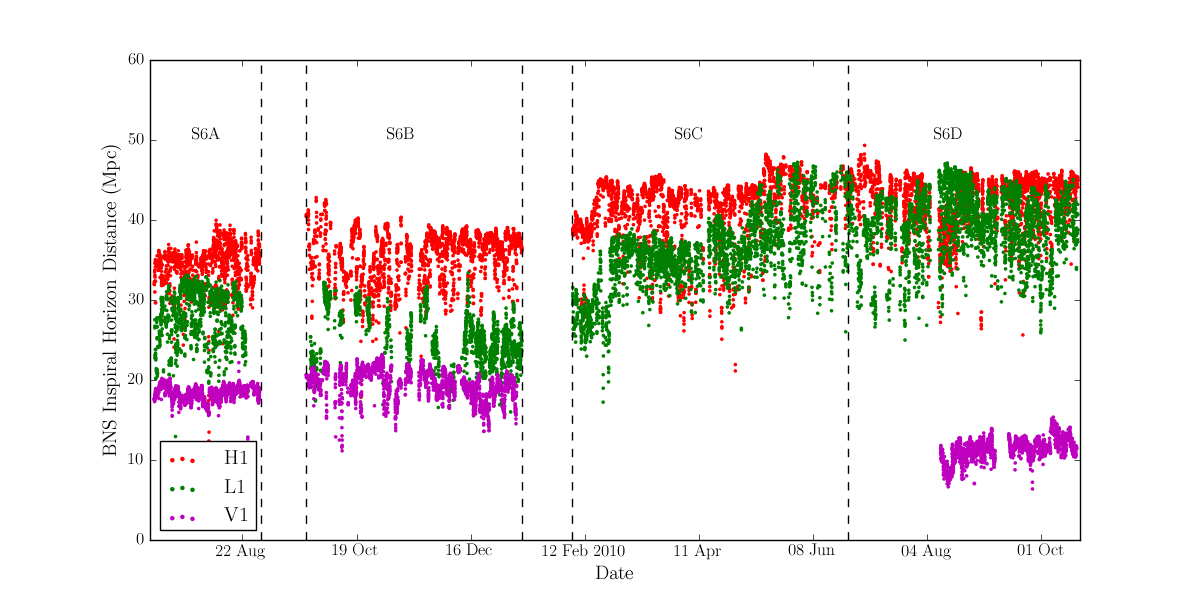
\includegraphics[width=9in]{figures/s6-hzrange_v_time.png}
\end{center}
\caption{The inspiral range for a $1.4/1.4\,\Msun$ \ac{BNS} system at \ac{SNR} $8$ in each \ac{IFO} across \ac{S6}. The range is computed by \texttt{lalapps\_tmpltbank} using equation \ref{eqn:DtoRho}. Each dot represents the range in a $2048\,$s--long analysis chunk.}
\label{fig:s6_insprange_v_time}
\end{figure}
\end{landscape}

\clearpage

\begin{figure}[p]
\begin{center}
\label{fig:s6a_insprange}
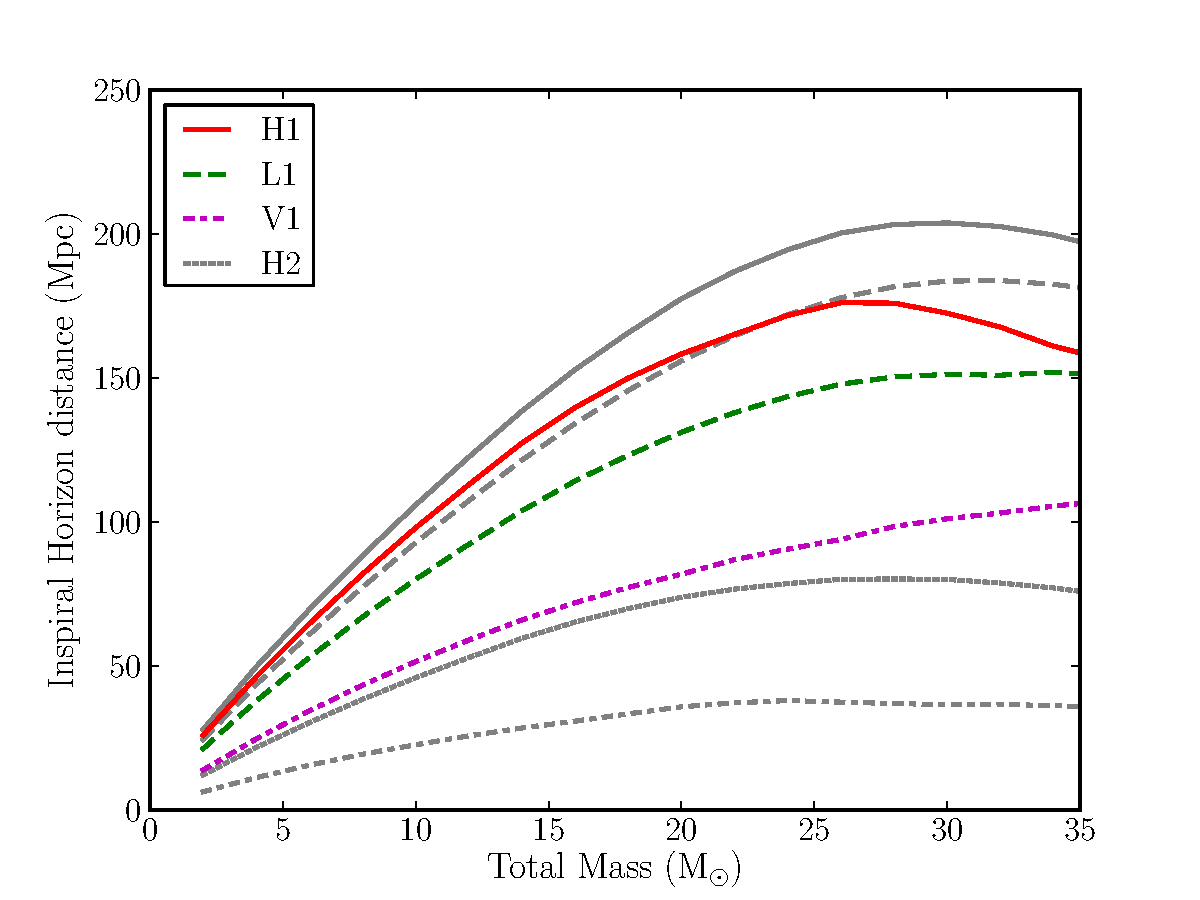
\includegraphics[width=6in]{figures/s6a_insprange.pdf}
\end{center}
\caption{Average inspiral range of S6A. Ranges were computed by \texttt{lalapps\_tmpltbank} using equation \ref{eqn:DtoRho} with $\rho=8$, then averaged over all analysis chunks in the epoch. S6 ranges are in color; best S5 ranges are in gray. Although H2 was not used in \ac{S6}, it is shown for comparison to V1.}
\end{figure}

\begin{figure}[p]
\begin{center}
\label{fig:s6b_insprange}
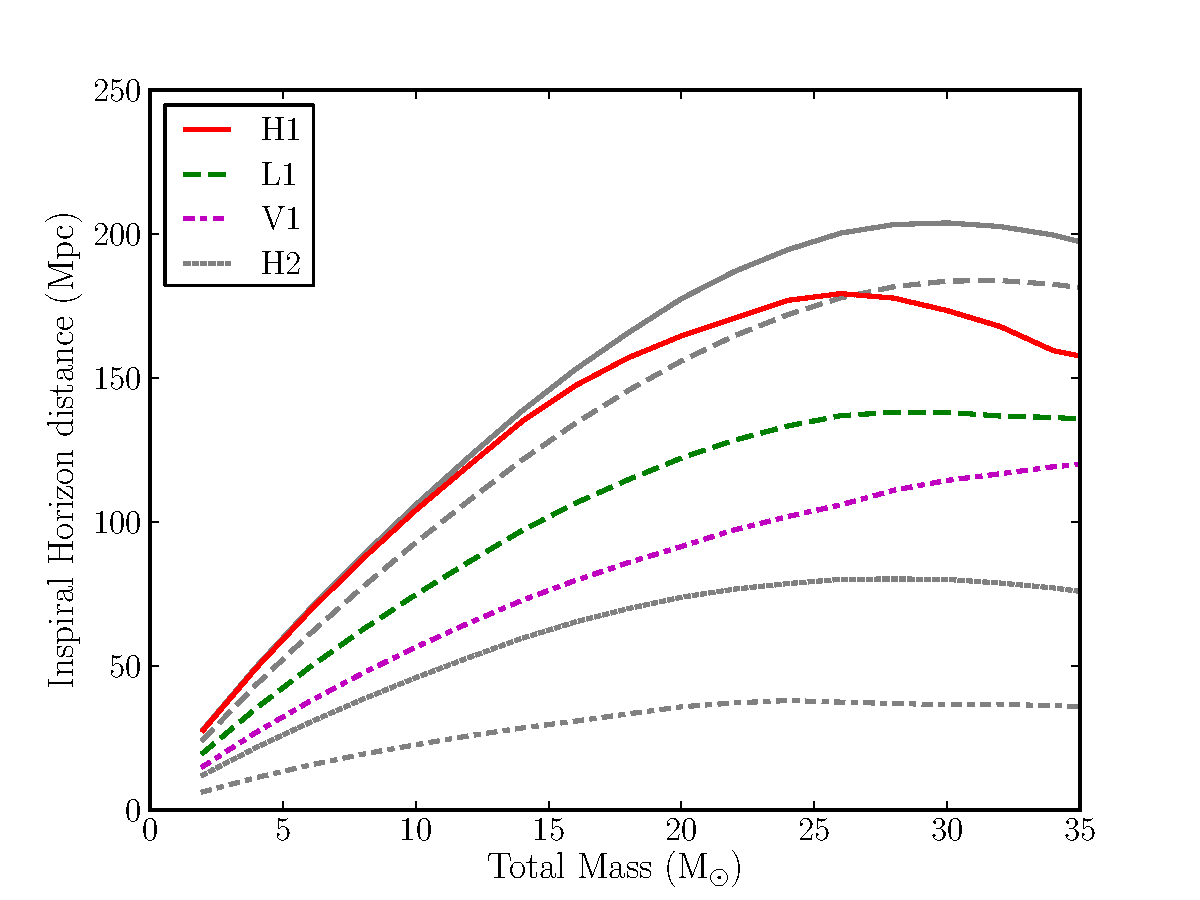
\includegraphics[width=6in]{figures/s6b_insprange.pdf}
\end{center}
\caption{Average inspiral range of S6B. Ranges were computed using the same method as in Figure \ref{fig:s6a_insprange}.}
\end{figure}

\begin{figure}[p]
\begin{center}
\label{fig:s6c_insprange}
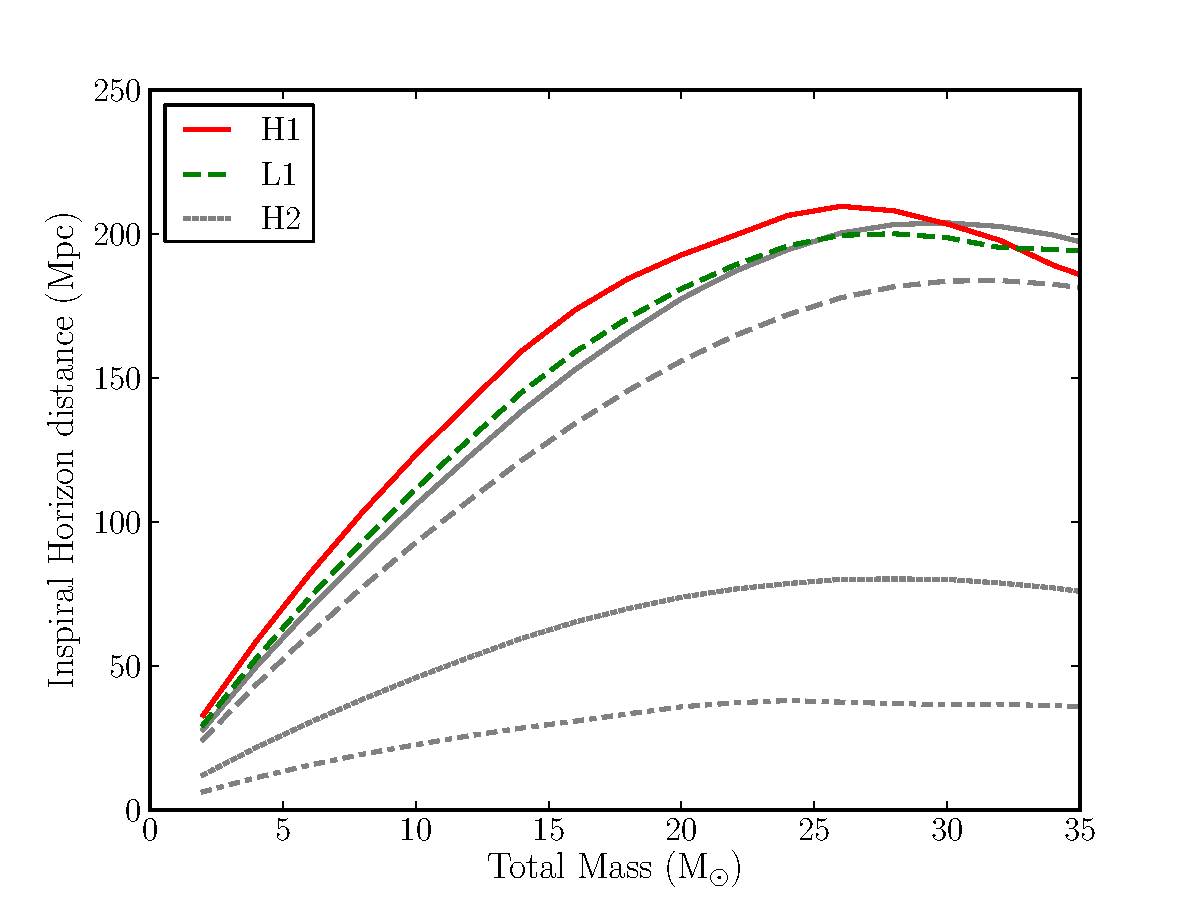
\includegraphics[width=6in]{figures/s6c_insprange.pdf}
\end{center}
\caption{Average inspiral range of S6C. V1 is not shown as it was down for commissioning during this period. Ranges were computed using the same method as in Figure \ref{fig:s6a_insprange}.}
\end{figure}

\begin{figure}[p]
\begin{center}
\label{fig:s6d_insprange}
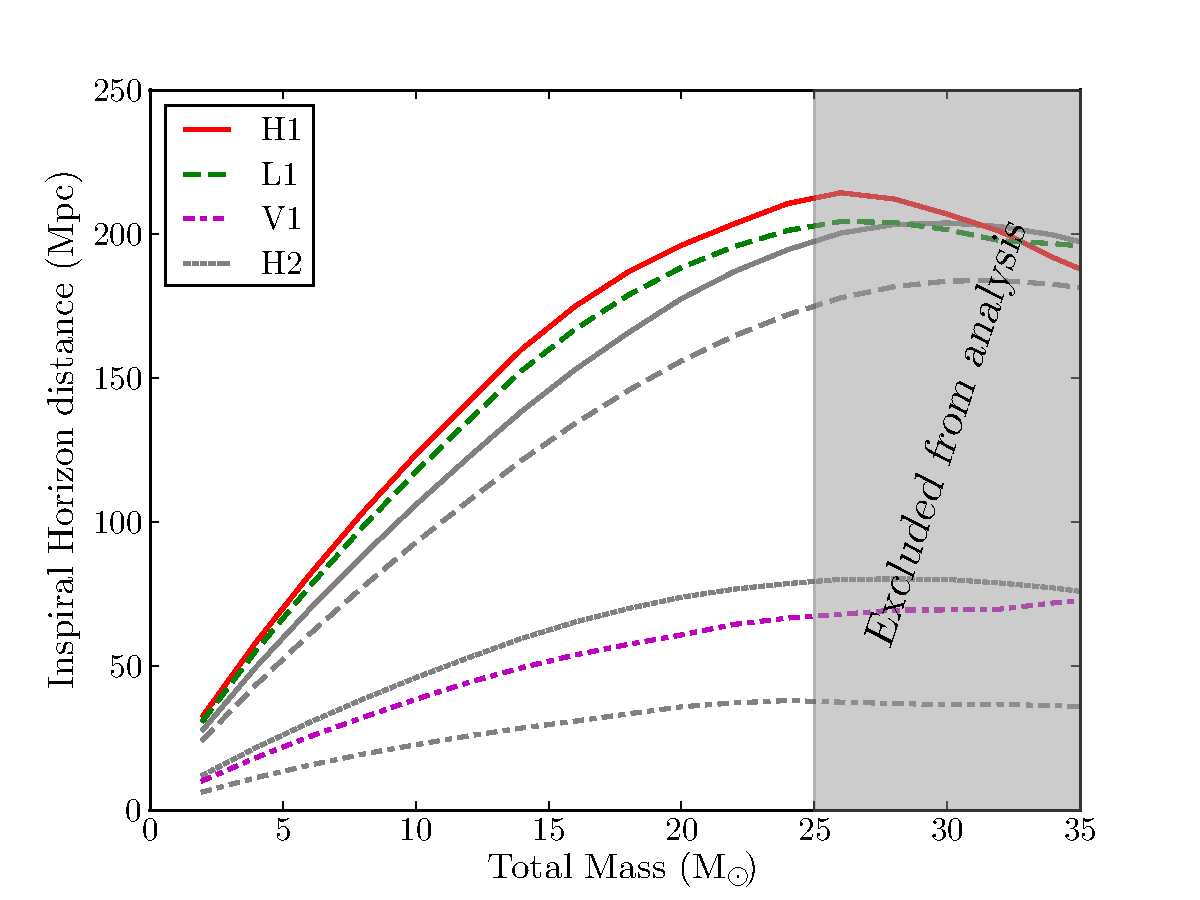
\includegraphics[width=6in]{figures/s6d_insprange_alt.pdf}
\end{center}
\caption{Average inspiral range of S6D. Shaded region indicates the mass range that was excluded in the low mass search for this period. Ranges were computed using the same method as in Figure \ref{fig:s6a_insprange}.}
\end{figure}

\subsection{S6A}
\label{sec:s6a}

At the start of the S6 Science run, the \ac{LIGO} detectors had lower
sensitivity and more glitches than in later epochs. This can be seen in Figure
\ref{fig:s6_insprange_v_time}. In fact, the S6A \ac{LIGO} ranges were somewhat
lower than they had been during their peak sensitivity in \ac{S5}. Figure
\ref{fig:s6a_insprange} shows the average inspiral range versus binary total
mass during S6A as compared to best ranges of \ac{S5}. We can see that Virgo,
however, showed much improvement over VSR1.

In the joint LIGO and Virgo search that occurred during \ac{VSR1} and the last
five months of \ac{S5} (the ``S5-LV" search), false alarm rates (FARs) were
based on a likelihood statistic that took into account the relative
sensitivites of various interferometer combinations. The sensitivies were used
to apply a weighting factor to each coincidence type so that more senstive
detector combinations were promoted, allowing false alarm rates to be computed
once across all combinations (as opposed to using equal-weighted bins to
compute combined \acp{FAR} from uncombined, as described in Chapter \ref{far})
\cite{S5LowMassLV}. This was implemented for two main reasons: first, with both
H2 and V1 active, four interferometers had to be analyzed, which led to a large
number of coincidence types and coincident-detector times to consider. Second,
Virgo's sensitivity was much lower than the \ac{LIGO} detectors in VSR1, and,
due to high amounts of low-frequency noise, its low-frequency cutoff had to be
set to $60\,$Hz. Thus its template bank was truncated to have a maximum chirp
mass of $\sim2.6\,\Msun$ \cite{S5LowMassLV}. The probability that various
coincidence types detected a \ac{GW} was therefore far from equal, and so
re-weighting of triggers' \acp{SNR} needed to be applied. As can be seen in
Figure \ref{fig:s6a_insprange}, however, the range of V1 was substantially
better in \ac{VSR2} --- better than H2 --- and we were able to lower its
low-frequency cutoff so that it could cover the same mass range as \ac{LIGO}.
Essentially, V1 in S6 had taken the place of H2 in S5. Further, since V1 was
not co-located with the other detectors, we could slide all the instruments
against each other, which allowed us to analyze all instrument times. (Recall
from the last chapter that H1 and H2 could not be slid against each other
because they were co-located, and so H1H2-coincident time could not be
analyzed.) For these reasons, and the fact that the \ac{S5}-LV likelihood
method was still being developed when S6A started, we decided to analyze
\ac{S6} in the same manner as in the \ac{S5} search described in Chapter
\ref{ch:s5_results} (the ``12-18 month search"\footnote{The name 12-18 month
comes from the fact that that search covered months 12 to 18 of S5.}), using
combined \ac{FAR} as our ranking statistic, and with all the coincidence types
being given equal weight. We also used many of the same tuning parameters as
the \ac{S5} 12-18 month search: the \ac{SNR} cut, $\chi^2$ and $r^2$ veto
thresholds, chirp-mass bins, and size of the e-thinca parameter\footnote{See
chapters \ref{ch:pipeline_principles} and \ref{ch:far} for definitions of these
parameters.} all remained the same.

There were a few minor adjustements, however. As mentioned in Chapter
\ref{ch:pipeline_principles}, we switched to using 3.5 restricted \ac{pN}
templates, although the template bank metric was still calculated using the
2\ac{pN} approximation. New \ac{SNR} was implemented as our ranking statistic
for computing uncombined \acp{FAR} after it was noticed --- in the 12-18 month
search and the S6A \ac{CBC} high-mass search\footnote{Recall from Chapter
\ref{ch:introduction} that the \ac{CBC} high-mass search covers the mass ranges
$25 \leq \mtotal/\Msun \leq 100$} --- that effective \ac{SNR} tended to
over-weight triggers with statistically low $\chi^2$ values. Pipedown replaced
older, more cumbersome, scripts to do post-\hipe~processing. As discussed in
Chapter \ref{ch:ihope_pipeline}, we decided to do coincidence clustering within
each chirp-mass bin as opposed to across all bins, as done in the 12-18 month
search. We also switched algorithms for computing combined \acp{FAR} from the
method discussed in section \ref{sec:alternate_cfar_method} of Chapter
\ref{ch:far} to using slide triggers' uncombined \acp{FAR}, discussed in
section \ref{sec:far-multiple_templates}. This change had little effect on the
analysis, as they are equivalent. In the 12-18 month search, \ihope~was run on
month-long blocks of data as opposed to the year-long block used in the \ac{S5}
first-year search. As discussed in Chapter \ref{ch:s5_results}, the duration of
\ihope~analysis periods were decreased to better reflect changing detector
behavior. We continued this trend of decreasing the analysis periods in
\ac{S6}: in S6A we decided to run \ihope~in week-long periods, with a different
analyst being in charge of each analysis period. Thus, S6A was (initially)
broken into 8 week-long runs.

Initially we also planned to use TrigScan clustering\footnote{See section
\ref{sec:first_inspiral} in Chapter \ref{ch:ihope_pipeline} for a description
of TrigScan clustering.} in \verb|lalapps_inspiral|\footnote{Recall from
Chapter \ref{ch:ihope_pipeline} that \texttt{lalapps\_inspiral} is the program
we use to perform match filtering.} to cluster triggers across templates.
However, we were surprised to find that trigger rates were much higher than in
\ac{S5}. TrigScan clustering was unable to keep the rate low-enough for many
\texttt{inspiral} jobs to finish (recall from Chapter \ref{ch:ihope_pipeline}
that a disadvantage of trigscan is that it cannot garauntee a maximum trigger
rate). Many jobs took several days to complete, or would simply run out of
memory. As a result, only two weeks out of the eight were able to finish with
TrigScan. Figure \ref{fig:avg_rate_per_tmplt} shows a comparison of the average
trigger rate-per-template between one of the weeks that finished (``S6aWk3")
and one of the months from the \ac{S5}-LV analysis (``lvMonth8") at each stage
of the pipeline. The rate was clearly higher for both H1 and L1 at all stages
in the pipeline. In particular, the rate at second inspiral (2 on the x-axis)
was not much lower than first inspiral (0 on the x-axis), implying that
$\chi^2$ was being calculated for a large number of triggers.\footnote{Refer to
Chapter \ref{ch:ihope_pipeline} for a description of each of these steps in the
\ihope~pipeline.} As this comparison had to use one of the weeks that finished,
the other weeks that did not finish most likely had an even higher rate as
compared to \ac{S5}.

To mitigate the high rates we decided to switch from TrigScan to time-window
clustering, discussed in section \ref{sec:first_inspiral}. What size window to
use was an open question and so we used the two weeks that completed to
investigate various clustering windows. We aimed to find the smallest window
that allowed the search to continue, and that resulted in the most efficient
recovery of vetoes. Three windows were considered: $10\,$ms, $30\,$ms, and
$100\,$ms. The $10\,$ms window was found to be too short: the trigger rates
were still too high for many runs to complete. This left the $30\,$ms and
$100\,$ms windows. Figure \ref{fig:roc_cluster_windows} shows a ROC
plot\footnote{Refer to section \ref{sec:plotroc} for a description of ROC
plots.} using $30\,$ms and $100\,$ms clustering. Note that in this plot we also
considered raising the low-frequency cutoff to $65\,$Hz. As can be seen, the
$30\,$ms window with the standard $40\,$Hz low-frequency cutoff provided the
best results. We therefore decided to use the $30\,$ms clustering for all of
\ac{S6}. Why TrigScan clustering did not work as well is an open question. It
may have simply been due to the high trigger rate. Another possibility is the
switch from 2\ac{pN} to 3.5\ac{pN} templates somehow affected its ability to
properly cluster \cite{Pekowsky:thesis}. We plan to re-address this before
Advanced \ac{LIGO}.

\begin{figure}[p]
\center
\subfigure[H1]{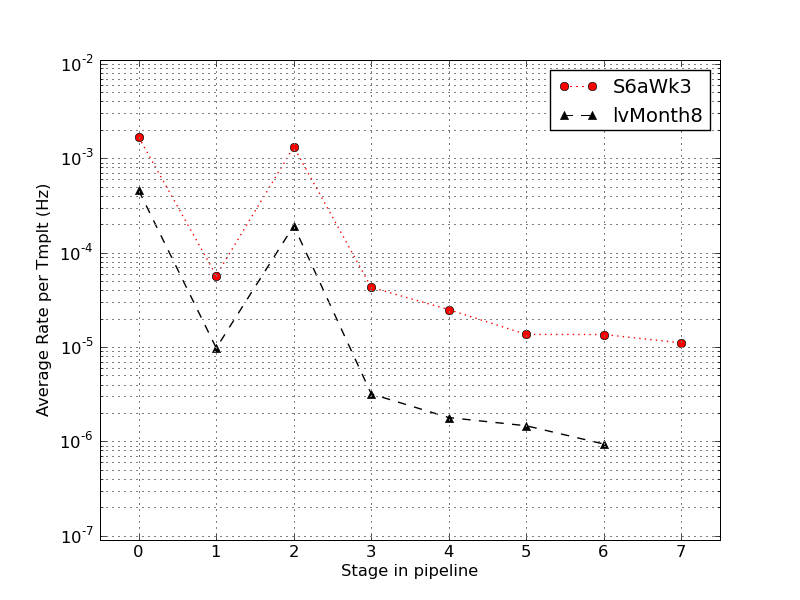
\includegraphics[width=2.8in]{figures/s6_clusterwin_investigation/H1_average_rate_per_tmplt_comparisons.png}}
\subfigure[L1]{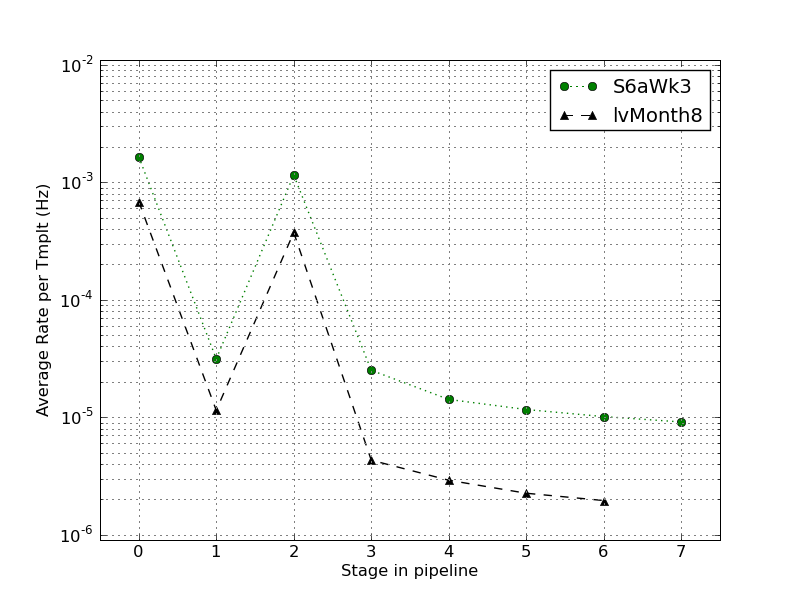
\includegraphics[width=2.8in]{figures/s6_clusterwin_investigation/L1_average_rate_per_tmplt_comparisons.png}}
\subfigure[V1]{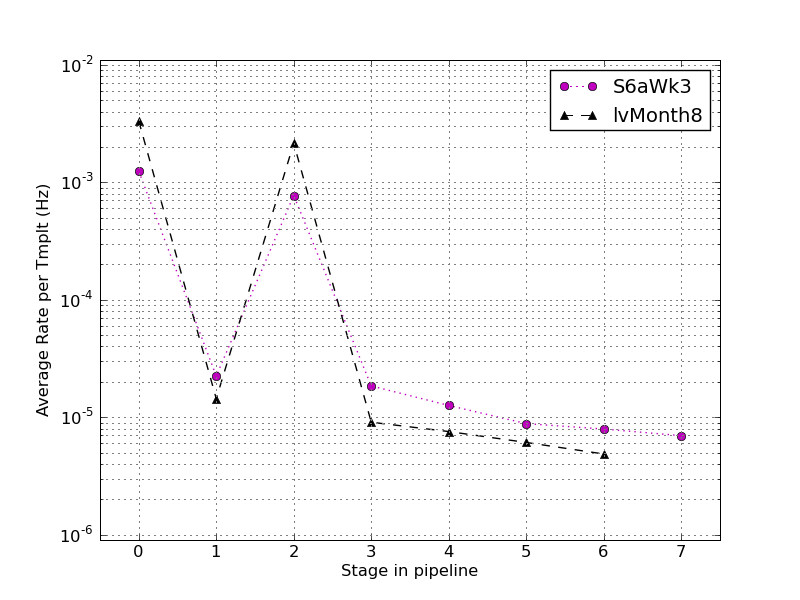
\includegraphics[width=2.8in]{figures/s6_clusterwin_investigation/V1_average_rate_per_tmplt_comparisons.png}}
\label{fig:avg_rate_per_tmplt}
\caption{The average trigger rate per template in week 3 of S6A as compared to
one month from the S5-LV analysis. Each point represents a different stage in
the pipeline: $0 \rightarrow$ \texttt{INSPIRAL\_FIRST}, $1 \rightarrow$
\texttt{THINCA\_FIRST}, $2 \rightarrow$ \texttt{INSPIRAL\_SECOND}, and $3
\rightarrow$ \texttt{THINCA\_SECOND}. (See Chapter \ref{ch:ihope_pipeline} for
a description of each of these stages.) Stages $4$--$7$ represent the
higher-category vetoes being applied at \texttt{THINCA\_SECOND}; there is an
extra stage in S6A because hardware injections were removed by an extra
veto-category (between steps $5$ and $6$), whereas in the LV search hardware
injections were removed as a part of the CAT2 vetoes (at step $4$).}
\end{figure}

\begin{figure}[p]
\label{fig:roc_cluster_windows}
\center
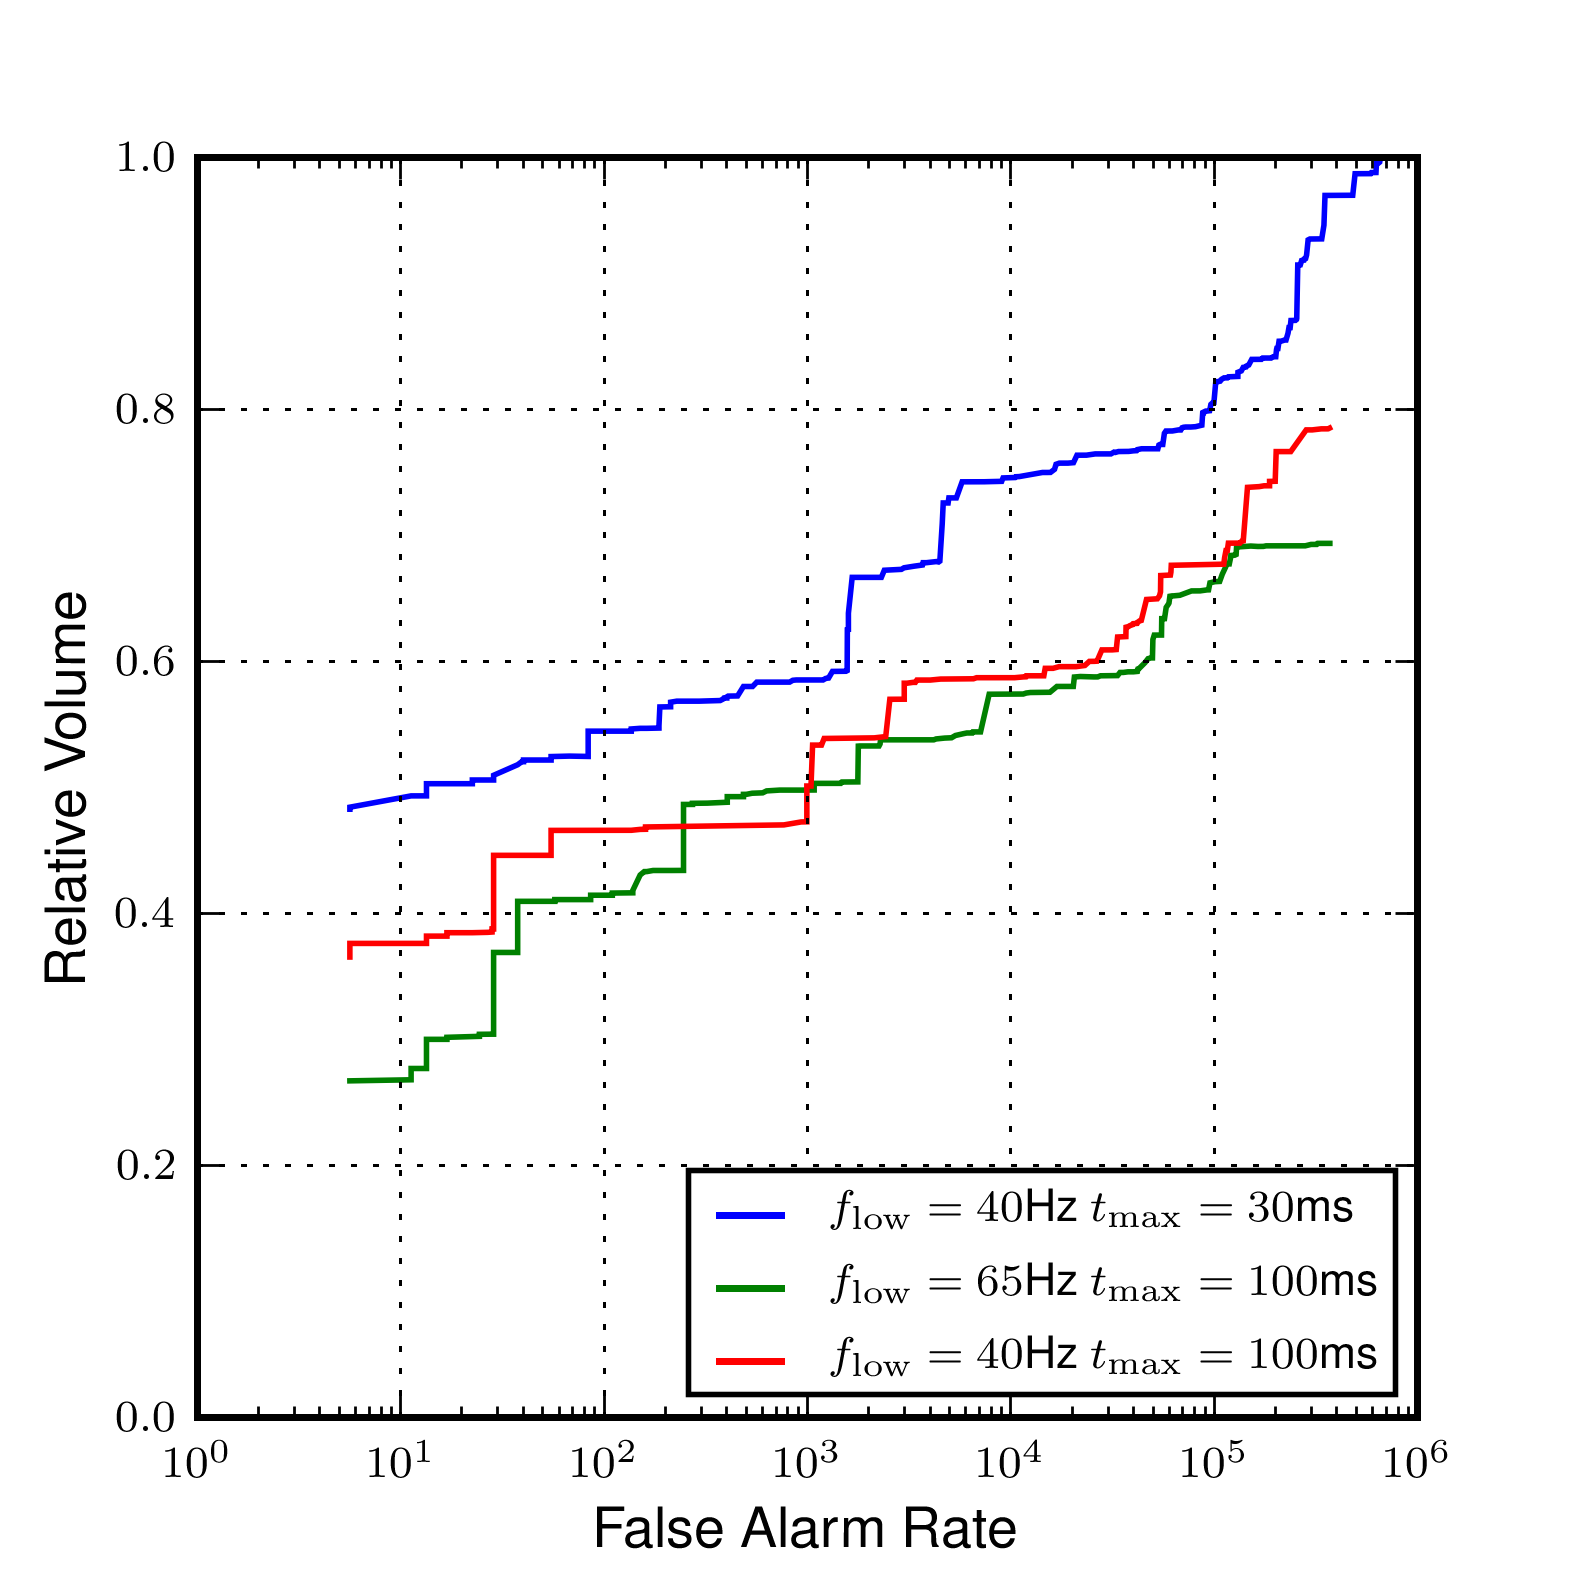
\includegraphics[width=5in]{figures/s6_clusterwin_investigation/s6week3cat4_ROC.png}
\caption{ROC plot from week 3 of S6A using various clustering windows and low-frequency cutoffs.}
\end{figure}

\subsection{S6B}
\label{sec:s6b}

S6B began after the commissioning break in September of 2009. While the
sensitivity in H1 improved slightly, the sensitivity in L1 was lower than in
S6A. Further, due to inclement weather, L1 struggled to stay in Science mode
for most of the period, and so the duty cycle was much lower. As stated above,
S6B ran from September to January. Fall brings a number of storms to the Gulf
of Mexico, resulting in increased \emph{microseismic} ($0.1$--$0.35$ Hz) noise.
The effects of this noise can be seen in Figure \ref{fig:s6_insprange_v_time}:
note that L1 is off for large periods of time, and that it has lower
sensitivity when it is in Science mode.

To mitigate the seismic problem at Livingston Hydraulic External Pre-Isolation
(HEPI) feed-forward was developed during S6B. Many of the interferometer's
optics sit on tables housed in vacuum chambers. These chambers are situated on
hydraulic actuators, which are used to actively dampen seismic noise. In the
feed-forward process, the output from seismometers on the floor were fed into
the actuators to cancel out the seismic motion \cite{Lundgren:personal-comm}.
The digital filters used in the feed-forward were implemented and tuned across
S6B. This led to L1 becoming more stable, allowing for longer Science mode
periods. The effect can be seen in Figure \ref{fig:s6_insprange_v_time}: a few
days prior to 16 December L1 begins to stay in Science mode for longer periods
of time. The increased stability eventually also allowed the laser power to be
increased to $14\,$W\footnote{The laser power was set to $14\,$W at both H1 and
L1 during the evening and on weekends --- when there was little seismic noise
from human activity --- throughout S6C and D. During working hours, the laser
was typically set to $10\,$W.} which in turn led to better
range.\footnote{Recall from Chapter \ref{ch:theory}, increasing laser power
decreases shot noise.}

Due to the sensitivity of the \ac{LIGO} detectors and L1's low duty cycle, we
decided to analyze S6B in three analysis periods. The first lasted from the
start of S6B until 11 November 2009, at which point the detectors were
re-calibrated. The second and third periods ran from 11 November to 11
December, and 11 December to 11 January, respectively. We chose 11 December to
end the second period so that each period was approximately the same duration.

\subsection{S6C}
\label{sec:s6c}

After V1 went offline in January of 2010, another commissioning break was taken
to improve the sensitivity of the \ac{LIGO} detectors. Thus the S6C analysis
began approximately two weeks after the end of S6B, on 6 February. As can be
seen in Figures \ref{fig:s6_insprange_v_time} and \ref{fig:s6c_insprange}, the
commissioning throughout S6A and B paid dividends during S6C and D: it was
during these periods that the \ac{LIGO} detectors reached their peak
sensitivity, surpassing that of \ac{S5}.

It was during S6C that Pipedown was completed.\footnote{Pipedown was used
throughout S6A and B. However, for both of those periods, it could only produce
tables of loudest zero-lag events and IFAR plots. An early form of the
\ihope~page and loudest-events table was used for S6A. For S6B injection
finding, \texttt{PrintMissed}, and \texttt{PrintSims} tables were added. By
S6C, loudest-slide tables were added along with \texttt{PlotFM} plots.} This
allowed us to perform studies to improve the sensitivity of the search that
used the loudest coincident-triggers from time-slides (\emph{loudest-slide
studies}). New data-quality tools were also finished, including daily
\ihope~\cite{Pekowsky:thesis} and a DQ wiki page. This page, which was
generated each week, brought together information from online analyses and veto
tools, including daily \ihope, an online excess-power search (Omega), ``hveto"
(for \emph{Hierarchical Veto}, this is a tool that hierarchically ranks various
auxillarily channels as potential vetoes by the significance of the correlation
between the vetoes and triggers from the \ac{GW} channel \cite{Smith:hveto}),
and UPV (for \emph{Used Percentage Veto}, this is a tool that looks for
correlations between auxilarilly channels and the \ac{GW} channel; if a channel
is strongly coupled for a set of triggers, it is used as a veto
\cite{Isogai:UPV}). We therefore implemented the following system to analyze
the data:
\begin{itemize}

\item{Each week a different analyst would be assigned to complete the \ac{DQ}
study. This involved examining the DQ page for that week and checking the e-log
for potential issues that would affect the \ac{CBC} analysis. The analyst would
record their findings on the DQ page (as this page was a wiki, it could be
edited after it was generated) and then present them on a weekly teleconference
devoted to the S6 analysis.}

\item{A ``lead" analyst would run \ihope~on two weeks' worth of data, with a
``second" providing support (e.g., if the lead could not make a teleconference
or had difficulty getting the analysis to complete, the second would provide
help). We required that the lead analyst be one of the two people who performed
the DQ study for one of the weeks that the \ihope~run covered. Thus the analyst
would be intimately familiar with potential issues in his or her run.}

\item{The lead or second would generate a blinded \ihope~page\footnote{Recall
from section \ref{sec:ihope_page} that a ``blinded" page is one that only
presents results from playground-analysis time and injections. An ``unblinded"
page is one in which all data from all times is presented.} after
\ihope~completed (typically a few days). We would look over the page on the S6
teleconference, paying careful attention to loudest-slide events and nearby
missed injections. We were particularily interested in slide events that had
combined New \acp{SNR} greater than $11.3$ as this would prevent detecting a
\ac{GW} with a \ac{SNR} of $8$ in each detector.\footnote{Recall from section
\ref{sec:coincidence_test} that combined New SNR is calculated from the
quadruture sum of the single-detector triggers. If a loudest-coincident trigger
had a combined New SNR greater than 11.3, all zero-lag triggers would have a
false alarm rate of at least 1 per few years. We cannot claim statistical
confidence that a zero-lag trigger was from a GW signal with a FAR that large.}
The DQ studies would be reviewed to see if any flags or events recorded in the
e-logs could explain the loudest slides. If a flag was found that passed safety
checks --- i.e., it did not veto injections --- it would be added to the
collection of vetoes used by the search as either a category 2 or category 3
veto. UPV vetoes were also added at this point, as category 3 vetoes. The lead
or second would then re-run the second coincidence stage and Pipedown with
these new vetoes (this typically took a few hours). The new blinded \ihope~page
would be checked again to make sure no new vetoes could be derived and that
there were no glaring problems. An unblinded page would then be generated and
presented on the full \ac{CBC} teleconference to see if there were any \ac{GW}
candidates.}

\item{This process would be repeated on successive weeks, with each new
analysis using the updated vetoes from the previous two weeks. The analysis was
thereby fine-tuned as S6C continued.}

\end{itemize}

This method of using loudest slide triggers resulted in a number of vetoes
being generated specifically for the low-mass \ac{CBC} search. Many of these
vetoes were only used once, as they were based on a specific event that
occurred at one of the detectors, such as a computer malfunctioning on a
paritcular day. However, the study did result in several long-term vetoes being
implemented. Section \ref{sec:seismic_veto} gives an example of one of these
vetoes. Routinely unblinding the analysis also decreased the latency between
when data was taken and when results were obtained. By the end of S6C and
throughout S6D we were unblinding results and checking for GW signals
approximately two weeks after the data had been taken. 

We decided to decrease the mass-range of our template bank to $2 \leq
\mtotal/\Msun \leq 25\,\Msun$ at the end of S6C, based on results obtained
during that epoch. This decision to change the upper-mass limit of the bank was
influenced by two observations: first, we found that the templates in the
$25$--$35\,\Msun$ range frequently created triggers with relatively large New
SNR when a glitch existed in the data. Nearly half of the top 10 loudest events
came from this part of the template bank in each of the two week periods,
despite it covering less than a third of the total mass space. The
loudest-slide events in the medium and high chirp-mass bins were also largely
dominated by this mass range. The other factor leading to the decision was that
the high-mass \ac{CBC} search, which covers the mass range $25 \leq
\mtotal/\Msun \leq 100$, overlapped the low-mass search in this region. This
overlap was unneeded since the template placing algorithm in
\texttt{lalapps\_tmpltbank} would adequately cover the $\mtotal = 25\,\Msun$
line within each search. We therefore had two questions to answer: first, which
search was more sensitive to astrophysical GW signals in the $25$--$35\,\Msun$
region, the low-mass or the high-mass? Second, if the high-mass search was more
sensitive in this range, and we decreased the upper limit of the low-mass
search template bank, what would the effect on the low-mass search be?

To answer the first question, we ran the low-mass and high-mass search on the
same 3 weeks of data (weeks 11-14 of S6C) and then compared how well they
recovered injections in the overlap region ($\mtotal \in [25,35]\,\Msun$).
Figure \ref{fig:mass_investigation-plotfm_lowmass} shows the found/missed plot
as a function of total mass in the overlap region for the low-mass search, and
Figure \ref{fig:mass_investigation-plotfm_highmass} shows the same for the
high-mass search. The high-mass search appears to be more sensitive: more
injections are recovered at farther distances, and a few injections that were
missed in the low-mass search are now found. That the high-mass search is more
sensitive in the overlap region is further supported by Figure
\ref{fig:mass_investigation-plotroc}, which shows the ROC plot for injections
in the overlap region.\footnote{It is not surprising that the high-mass search
is more sensitive in this mass regiong. The high-mass search uses templates
that include the ``merger" part of a GW signal, whereas the low-mass templates
only include the ``inspiral" part of the signal. (Recall from Chapter
\ref{ch:theory} that merger occurs when the component masses pass the \ac{ISCO}
radius, at which point they plunge into each other.) Since \ac{ISCO} grows with
mass, and since GW-frequency goes as the inverse of the separation distance
(c.f. equations \ref{eqn:tau_0-a} and \ref{eqn:f_evolution}) high mass systems
merge at lower gravitational-wave frequencies. This means that higher binaries
will have fewer inspiral cycles and will merge in the frquency range to which
the LIGO and Virgo detectors are most sensitive.}

The high-mass search was clearly more sensitive in the overlap region,
suggesting we should decrease the upper limit of the mass-range covered by the
template bank of the low-mass search. To see the effect this might have on the
low-mass search, a test \ihope~analysis with a template bank covering the range
$2 \leq \mtotal/\Msun \leq 25$ was carried out over the first two weeks of S6C
and compared to the original run, which had the $2 \leq \mtotal/\Msun \leq 35$
template bank. Figure \ref{fig:smaller_bank_investigation-lowmass} shows the
found/missed plot as a function of chirp-mass for the two runs (spinning
injections are excluded in these plots). There are a few subtle differences.
Several injections on the edge of the range are found with lower \acp{FAR} with
the lower-bank. This is expected since the volume of parameter-space we are
searching is smaller, effectively giving a smaller trials factor.

Only one injection appears to have a lower false alarm rate in the analysis
with a lower-mass bank: the one with $\mchirp \approx 3.8\Msun$ and decisive
distance $\approx 18\Mpc$. In the analysis with $\mtotal \in [2,35]\Msun$ the
injection was ``found," albeit with a large combined \ac{FAR} (signified by the
orange dot in Figure \ref{fig:smaller_bank_investigation-lowmass-full_bank}).
In the analysis with $\mtotal \in [2,25]\Msun$ the injection was missed
(signified by the red cross). This injection never should have considered
``found" in the $\mtotal \in [2,35]\Msun$ analysis, however: a followup
investigation found that a glitch occurred during the injection. This glitch
created a trigger when match filtered with a high-mass template. Since
\texttt{ligolw\_inspinjfind} only uses a time-window to match injections with
triggers, it labelled the injection as ``found" even though the recovered
parameters were not close to the injected. In the $\mtotal \in [2,25]\Msun$
analysis, no templates match filtered with the glitch created triggers and so
the injection was considered missed, as it should have been. Thus, this
injections was another indication that the $2 \leq \mtotal/\Msun \leq 25$
template bank was better suited for the low-mass search.

Another metric of interest was the effect of using the $2 \leq \mtotal/\Msun
\leq 25$ template bank on the loudest-slide events. Table
\ref{tab:smalller_bank_investigation-loudest_slides} compares the three
loudest-slide triggers from the original run and from the new run. There was
little difference in the low and medium chirp-mass bins, but the high-mass bin
shows clear improvement. The loudest event in the high chirp-mass bin with the
$2 \leq \mtotal/\Msun \leq 35$ bank had a combined New \ac{SNR} of $11.78$
whereas with the smaller bank it is $9.64$. This means that an event in the
high chirp-mass bin with \ac{SNR} $8$ in each \ac{IFO} (the \ac{SNR} on which
we base projected detection capabilities) would now stick out above the
background.

Using a template bank with $2 \leq \mtotal/\Msun \leq 25$ offered clear
advantages and little or no disadvantages as compared to the bank with $\mtotal
\leq 35\Msun$. For this reason we decided that we should lower the upper limit
of the template bank to $\mtotal \leq 35\Msun$ for all subsequent analysis.
This decision was made as the analysis of the two weeks ending on 25 June 2009
was being completed. We therefore decided to stop S6C on that date, and begin
``S6D" with the analysis starting on 26 June using the $2 \leq \mtotal/\Msun
\leq 25$ template bank. It was suggested that we re-analyze all of the S6C
weeks with this new bank. However, given the relatively minor differences in
the found/missed plots, we decided against it. This decision was further
bolstered by Figure \ref{fig:smaller_bank_investigation-roc}, which shows a ROC
plot comparing the analysis with $\mtotal \leq 25\Msun$ to the analysis with
$\mtotal \leq 35\Msun$. The gain in relative volume was not considered large
enough to warrant a re-analysis.

\begin{figure}[p]
\center
\subfigure[Results using the low-mass search.]{\label{fig:mass_investigation-plotfm_lowmass}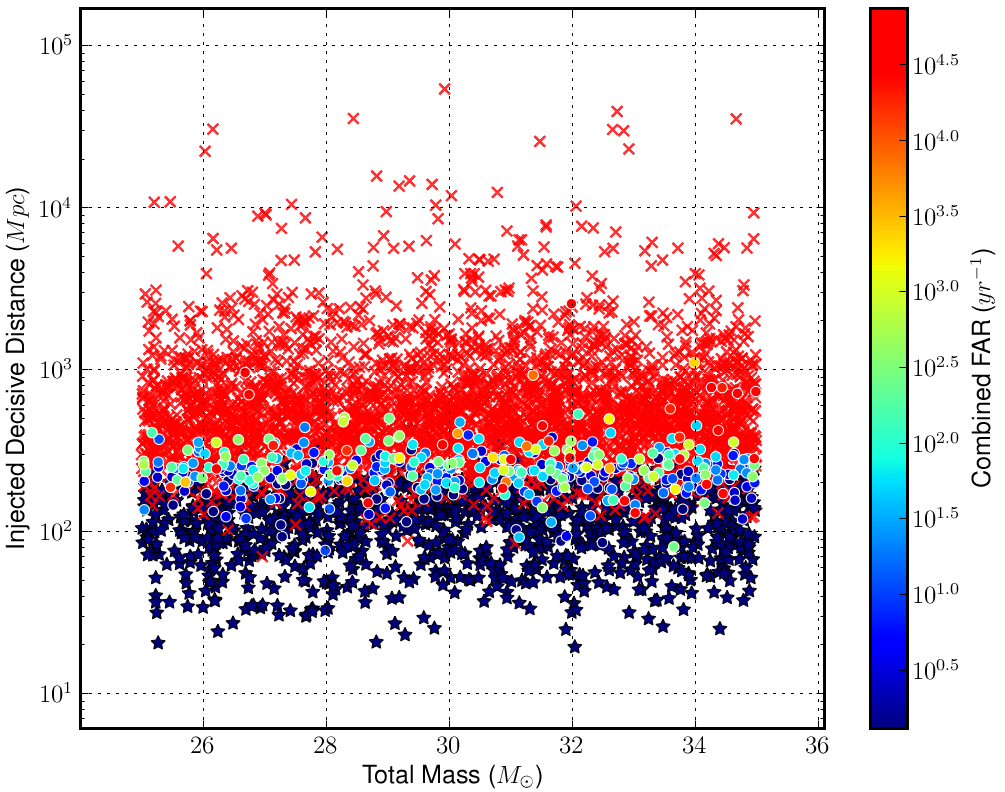
\includegraphics[width=4.7in]{figures/lower_tmpltbank_investigation/lowmass_plotfm.png}}
\subfigure[Results using the high-mass search.]{\label{fig:mass_investigation-plotfm_highmass}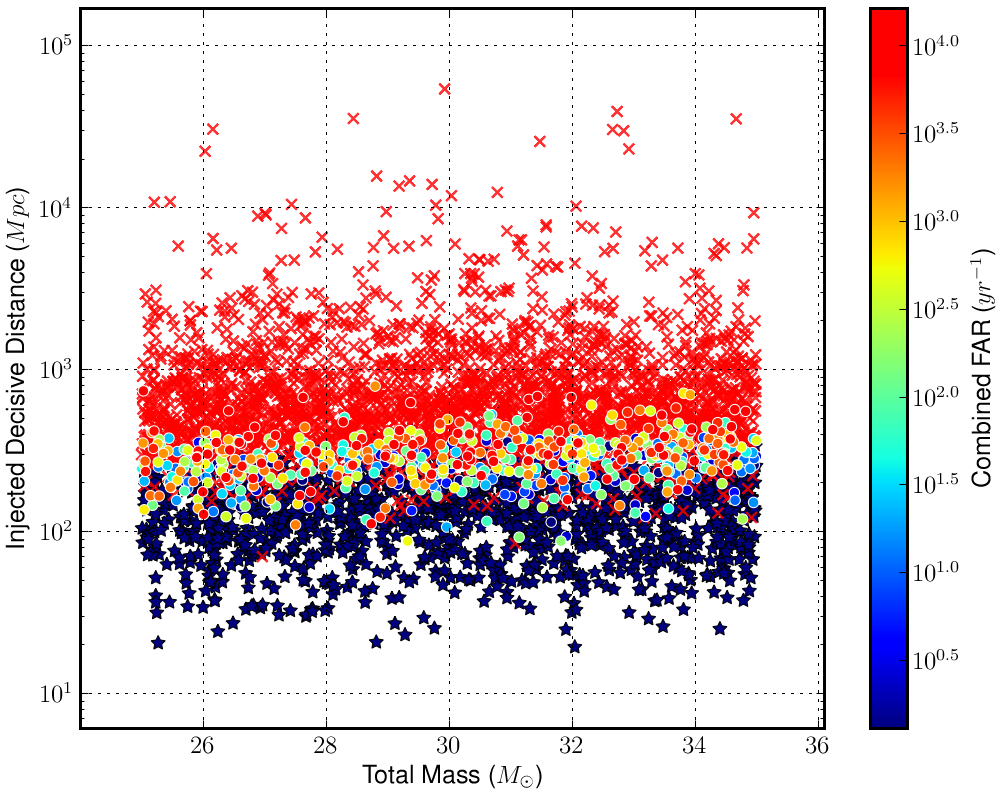
\includegraphics[width=4.7in]{figures/lower_tmpltbank_investigation/highmass_plotfm.png}}
\label{fig:mass_investigation-plotfm}
\caption{Found/missed plots as a function of total mass in the overlap region
($25 \leq \mtotal/\Msun \leq 35$) between the low-mass and high-mass search.
Plot generated by \texttt{ligolw\_cbc\_plotfm} by running on three weeks of S6C
data.}
\end{figure}

\begin{figure}[p]
\center
\label{fig:mass_investigation-plotroc}
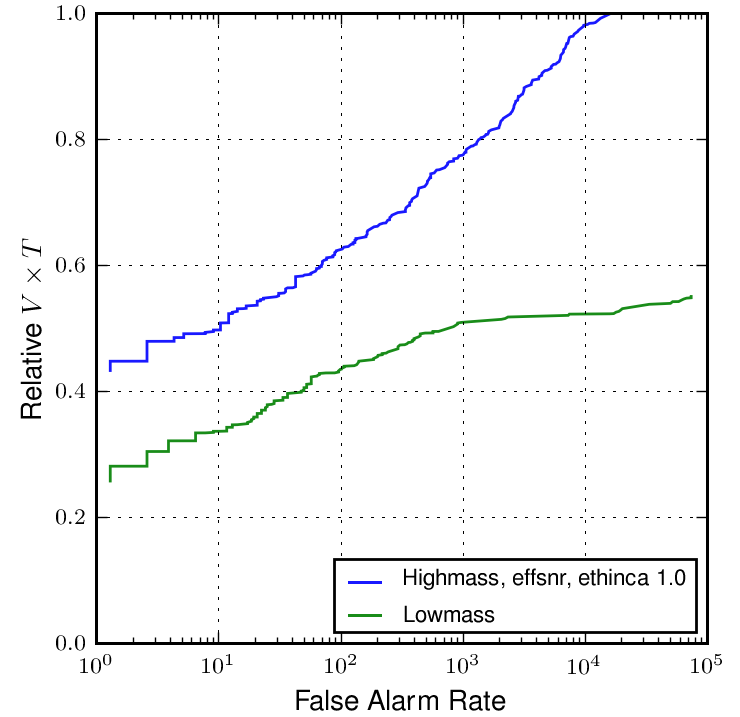
\includegraphics[width=5in]{figures/lower_tmpltbank_investigation/overlap_allinj_ROC.png}
\caption{ROC plot comparing the sensitive volume in the overlap region between
the low-mass and high-mass \ac{CBC} searches. All injection used for this plot
have $\mtotal/\Msun \in [25.0, 35.0]$. We see that the high-mass search has a
larger relative volume at all FARs, indicating it is more sensitive to GW
signals in this mass-range. For more details on ROC plots, see section
\ref{sec:plotroc}.}
\end{figure}

\begin{figure}[p]
\center
\subfigure[Results using the full bank.]{\label{fig:smaller_bank_investigation-lowmass-full_bank}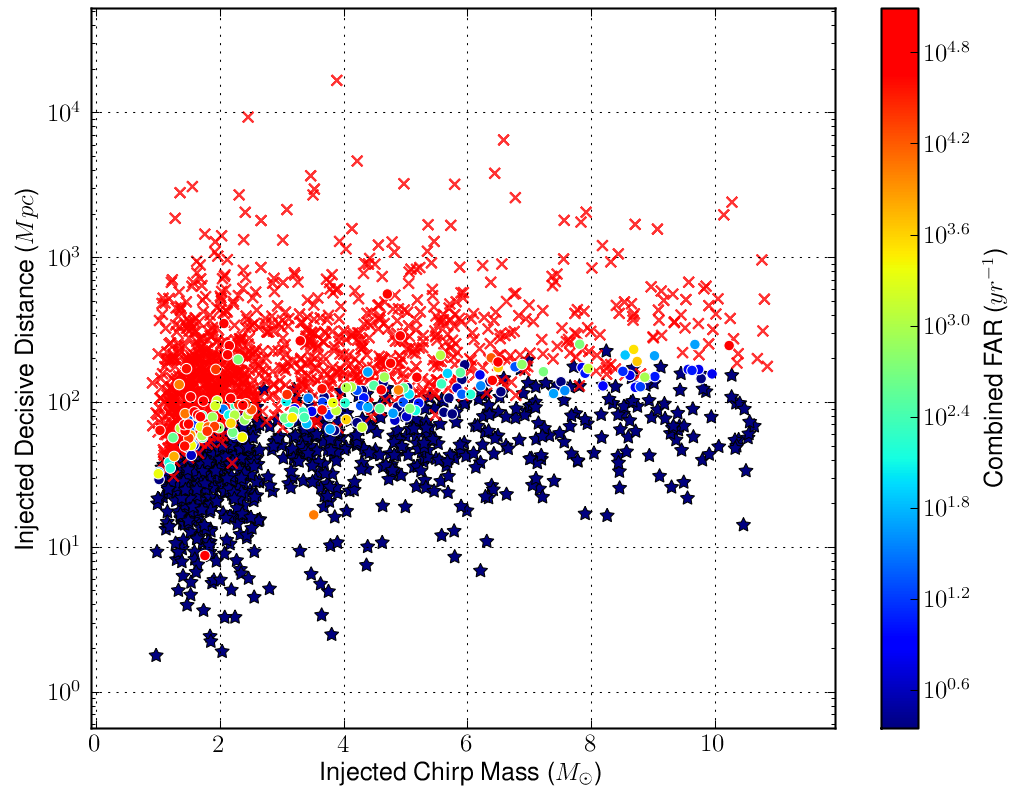
\includegraphics[width=4.8in]{figures/lower_tmpltbank_investigation/lowmass-plotfm_full_bank.png}}
\subfigure[Results using the reduced bank.]{\label{fig:smaller_bank_investigation-lowmass-small_bank}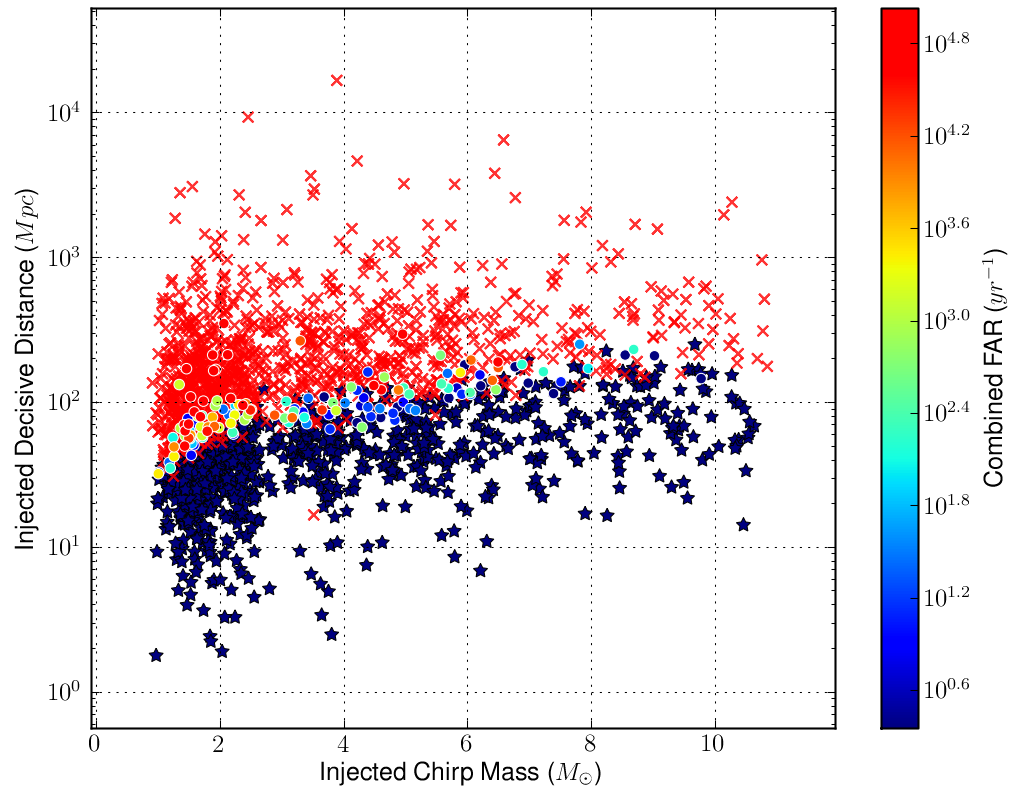
\includegraphics[width=4.8in]{figures/lower_tmpltbank_investigation/lowmass-plotfm_small_bank.png}}
\label{fig:smaller_bank_investigation-lowmass}
\caption{Found/missed plots as a function of total chirp mass. Both plots were
generated by \texttt{ligolw\_cbc\_plotfm} using the first two weeks of S6C
data. The top plot shows the results from using a template bank spanning $2
\leq \mtotal/\Msun \leq 35$ (``full" bank) and the lower plot shows the resuts
from using a $2 \leq \mtotal/\Msun \leq 25$ (``reduced" bank). Only
non-spinning injections with total mass $\leq 25\,\Msun$ were used in each
plot.}
\end{figure}

\begin{table}[p]
\label{tab:smalller_bank_investigation-loudest_slides}
\center
\begin{tabular}{| c | c | c | c | c |}
\hline
Chirp Mass Bin & Run & $\mchirp (\Msun)$ & $\mtotal (\Msun)$ & Combined New \ac{SNR} \\ 
\hline \hline
\multirow{2}{*}{Low} & Full Bank & 2.34 & 6.26 & 9.85 \\
                     & Reduced Bank & 2.68 & 10.37 & 9.81 \\
\hline
\multirow{2}{*}{Medium} & Full Bank & 5.36 & 18.88 & 10.63 \\
                        & Reduced Bank & 5.24 & 19.91 & 10.29 \\
\hline
\multirow{2}{*}{High}   & Full Bank & 12.87 & 29.61 & 11.78 \\
                        & Reduced Bank & 9.86 & 23.11 & 9.64 \\
\hline
\end{tabular}
\caption{Comparison of loudest slide events between low-mass \ac{CBC} runs, one
using the ``full" template bank ($2 \leq \mtotal/\Msun \leq 35$) and one using
the ``reduced" bank ($2 \leq \mtotal/\Msun \leq 25$). Results are taken from
the first two weeks of S6C data. The low, medium, and high chirp-mass bins are
defined as $\mchirp \in [0.0, 3.48), ~[3.48, 7.4),$ and $[7.4, \max(\mchirp)]$,
respectively, where $\max(\mchirp)$ is the largest possible chirp mass with
each bank.}
\end{table}

\begin{figure}[p]
\center
\label{fig:smaller_bank_investigation-roc}
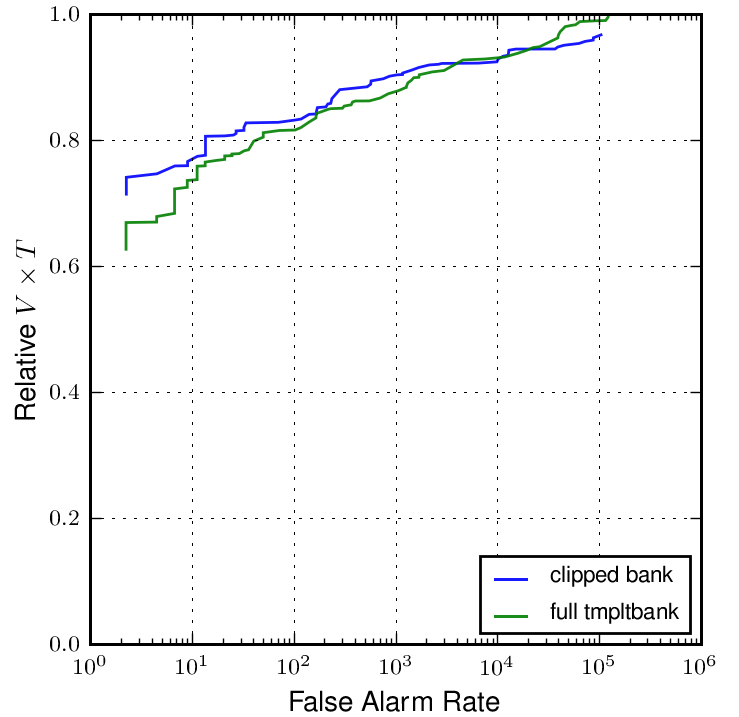
\includegraphics[width=5in]{figures/lower_tmpltbank_investigation/lowmass-lininj_compare_ROC.png}
\caption{ROC plot comparing the sensitive volume between the analysis using a
template bank that spanned $2 \leq \mtotal/\Msun \leq 25$ (here, labelled as
the ``clipped bank") and the analysis using a template bank that spanned $2
\leq \mtotal/\Msun \leq 35$. Only injections distributed uniformly in linear
distance were used in this plot; log-distributed injections showed similar
results.}
\end{figure}

\subsection{S6D}
\label{sec:s6d}

The method of analyzing data on two week periods that was pioneered during S6C
was continued throughout S6D. There were a few differences between S6C and D:
in addition to reducing the template bank, described above, we also implemented
two new automated vetoes: SeisVeto and a ``SNR $> 250$" flag. These are
discussed in more detail in sections \ref{sec:lvea_seismic} and
\ref{sec:spike_glitch}, respectively. The other major difference from S6C was
that VSR3 began during S6D.

Virgo came back online on 11 August 2009 to begin VSR3. As mentioned above, in
the break between VSR2 and VSR3, monolithic suspension was installed in an
effort to increase Virgo's range. Unfortunately, a mirror with an incorrect
radius of curvature was installed in the process. As can be seen in Figure
\ref{fig:s6_insprange_v_time}, this resulted in V1 having lower sensitivity
than it did in VSR2. The rate of non-Gaussian transient noise (glitches) was
also higher in V1 during VSR3.

Given Virgo's reduced sensitivity, we were concerned about leaving H1V1- and
L1V1-coincident triggers that occurred during H1L1V1-coincident time in the
data. As discussed in Chapter \ref{ch:far}, if we use all the possible
coincidence types\footnote{Recall that a ``coincidence type" refers to the
detectors contributed to a concident trigger. For example, if a trigger in H1
is coincident with a trigger in V1, then the coincidence type of the trigger is
H1V1. In H1L1V1-coincident time there are four possible coincidence types:
H1L1-, H1V1-, L1V1-, and H1L1V1-coincident triggers.} in H1L1V1-coincident
time, we have a trials factor of 12 (4 coincidence types $\times$ 3 chirp-mass
bins). This means that the combined \ac{FAR} of all (loud) triggers will be 12
times larger than the uncombined \ac{FAR}. In doing so we have treated all the
coincidence types with equal weight. However, with V1's reduced sensitivity, it
was far less probable that an H1V1- or L1V1-coincident trigger was a caused by
a GW than H1L1- or H1L1V1-coincident triggers. That the combined \acp{FAR} of
H1L1- and H1L1V1-coincident triggers would gain a factor of 12 due to the much
weaker H1V1- and L1V1-coincident triggers would clearly be an over-estimation
of the false alarm rate. The simplest fix was to simply remove H1V1- and
L1V1-coincident triggers in H1L1V1-coincident time. This would decrease the
trials factor in H1L1V1-coincident time to 6. Before doing this, however, we
investigated what the effect of removing these triggers would be. Namely, we
wanted to know if any injections would be missed, and we wanted to weigh this
against the decrease in \acp{FAR} for H1L1- and H1L1V1-coincident triggers.

In order to perform the study, two weeks of S6D/VSR3 data were used (from 3
September to 18 September 2010). Both \verb|ligolw_cbc_cluster_coincs| and
\verb|ligolw_cbc_cfar| have the ability to remove specific coincidence types
from a database; thus we simply re-ran \texttt{cFAR} on the Pipedown database
generated by the standard run to re-compute the combined \acp{FAR} with the
H1V1- and L1V1-coincident trigger in H1L1V1-coincident time excluded. 

Figure \ref{fig:V1doubles-found_missed-orig} shows the found/missed plot in
H1L1V1-coincident time for the ``original" analysis (with V1 doubles included);
Figure \ref{fig:V1doubles-found_missed-excluded} shows the same, but with the
V1 doubles excluded. Some injections do appear to be missed when the H1V1- and
L1V1-coincident triggers (``V1 doubles") are excluded. To get a better handle
on how many, and whether or not they are really ``found" injections (as opposed
to being a glitch within the injection-finding window), the plots in Figure
\ref{fig:V1doubles-coinc_types} were created. The top plot shows found/missed
injections in H1L1V1-coincident time as a function of coincidence type in the
original analysis (with V1 doubles included). There are clearly some injections
found as H1V1- and L1V1-coincident triggers, some of which are louder than all
time-slide (or ``background") coincidences. To get a sense of how many of these
triggers are actually due to injections (as opposed to being from a glitch that
occurred near the time of the injection), the bottom plot shows the accuracy of
the recovered chirp mass: triggers with a recovered chirp-mass fractional
accuracy $\sim0.0$ are most due to injections. When more detailed information
was printed for some of these injections, it was found that their effective
distance in V1 was lower than that in H1 or L1, meaning that, despite Virgo's
poor over-all sensitivity, there were still small areas in the sky to which V1
was more sensitive due to the relative antenna patterns of the detectors.

Still, the relative number of injections found as H1V1- and L1V1-coincident
triggers as compared to the number found as H1L1- or H1L1V1-coincident triggers
is clearly small. To weigh the gain in detecting these extra few injections
against the cost of doubling the trials factor, the ROC plot in  Figure
\ref{fig:V1doubles-roc} was created. This plot compares the relative sensitive
volume of leaving H1V1- and L1V1-coincident triggers in H1L1V1-coincident time
(blue curve) to excluding them (green curve). While the two curves are roughly
the same at high \acp{FAR}, removing the V1 doubles provides more sensitive
volume at lower \acp{FAR}, which is the region of most interest since we would
never claim a detection at the higher \acp{FAR}.\footnote{Also, recall from
section \ref{sec:plotroc} that ROC plots can be affected by injections being
mis-labelled as found if a glitch occurs near the time of the injection. This
occurs most often at high \acp{FAR}.} Note in particular that at lower \ac{FAR}
the green curve has approximately half the \ac{FAR} as the blue curve at the
same relative volume, as expected from the reduction in trials factor. Based on
these results and the small number of injections that would be missed, we
therefore decided to exclude H1V1- and L1V1-coincident triggers in
H1L1V1-coincident time from the analysis for S6D.\footnote{Note that we still
kept all triggers in H1V1- and L1V1-coincident time. Since these times are
mutually exclusive from H1L1V1- and H1L1-coincident time, leaving them in the
analysis had no effect on the \acp{FAR} of H1L1- and H1L1V1-coincident
triggers. Thus we only stood to gain by considering these times.}

\begin{figure}[p]
\center
\subfigure[H1V1 and L1V1 doubles included.]{\label{fig:V1doubles-found_missed-orig}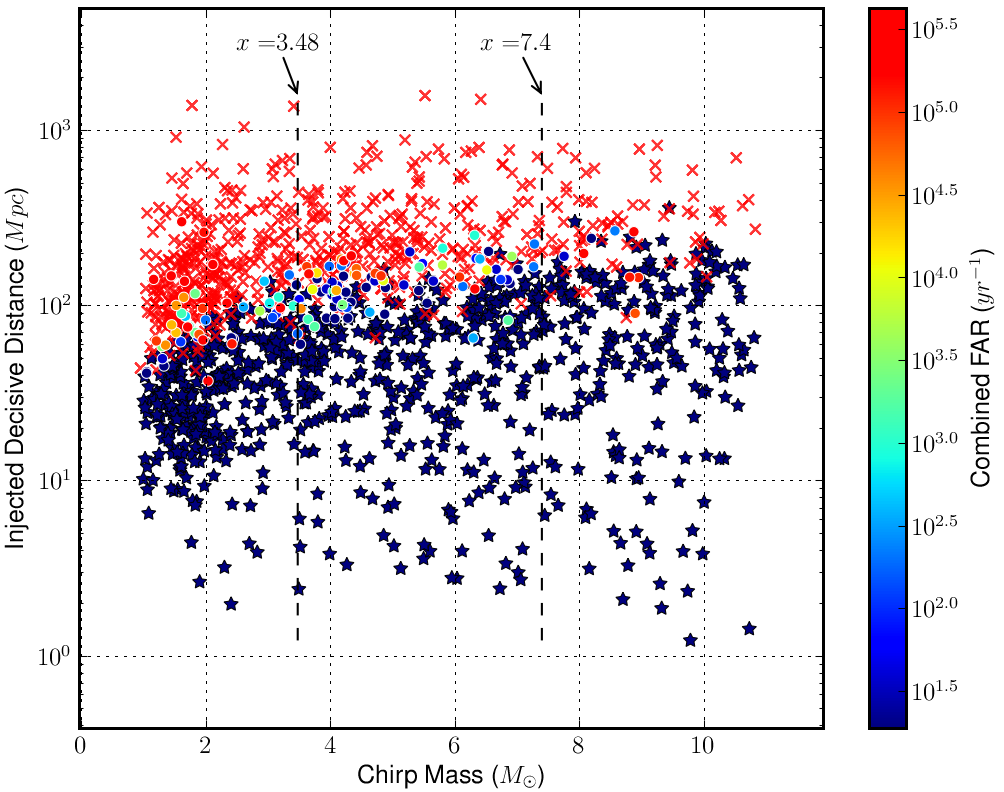
\includegraphics[width=4.8in]{figures/excluding_V1_doubles/plotfm_found_missed-orig.png}}
\subfigure[H1V1 and L1V1 doubles excluded.]{\label{fig:V1doubles-found_missed-excluded}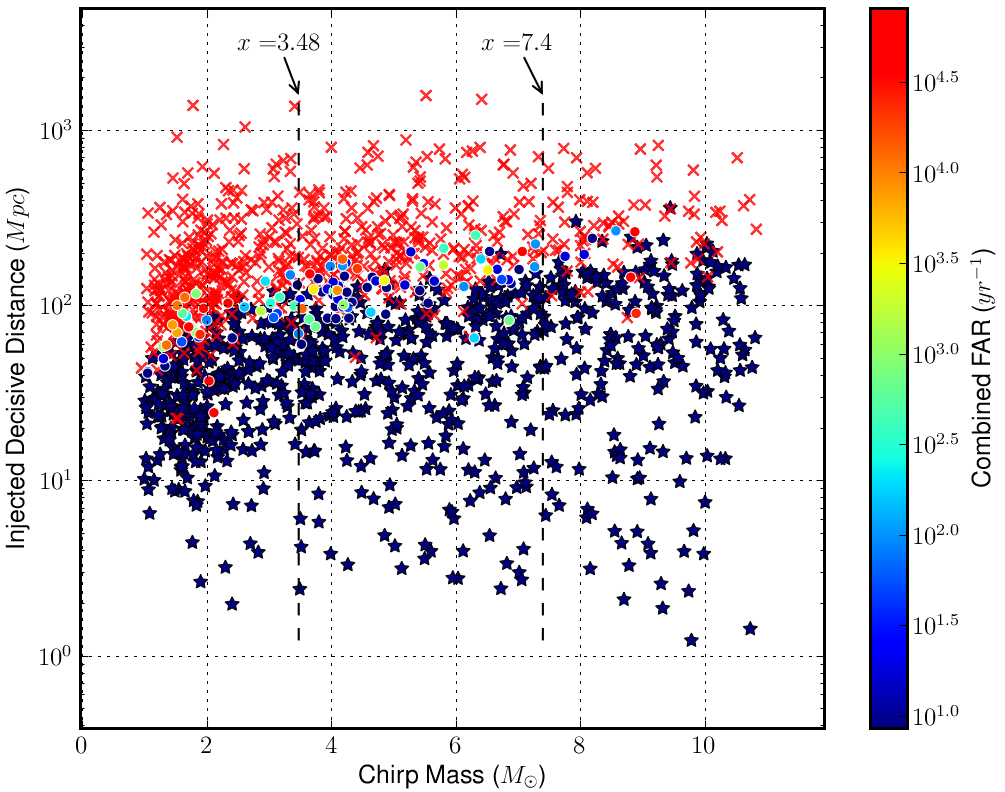
\includegraphics[width=4.8in]{figures/excluding_V1_doubles/plotfm_found_missed-excluded.png}}
\label{fig:V1doubles-found_missed}
\caption{Found/missed plots as a function of chirp mass in H1L1V1-coincident
time. The top plot includes H1V1- and L1V1-coincident triggers, the bottom plot
was created with H1V1 and L1V1 coincidences excluded. Both plots created by
\texttt{ligolw\_cbc\_plotfm} using two weeks of S6D/VSR3 data.}
\end{figure}

\begin{figure}[p]
\center
\subfigure[Decisive distance v. coincidence type.]{\label{fig:V1doubles-coinc_types-dist}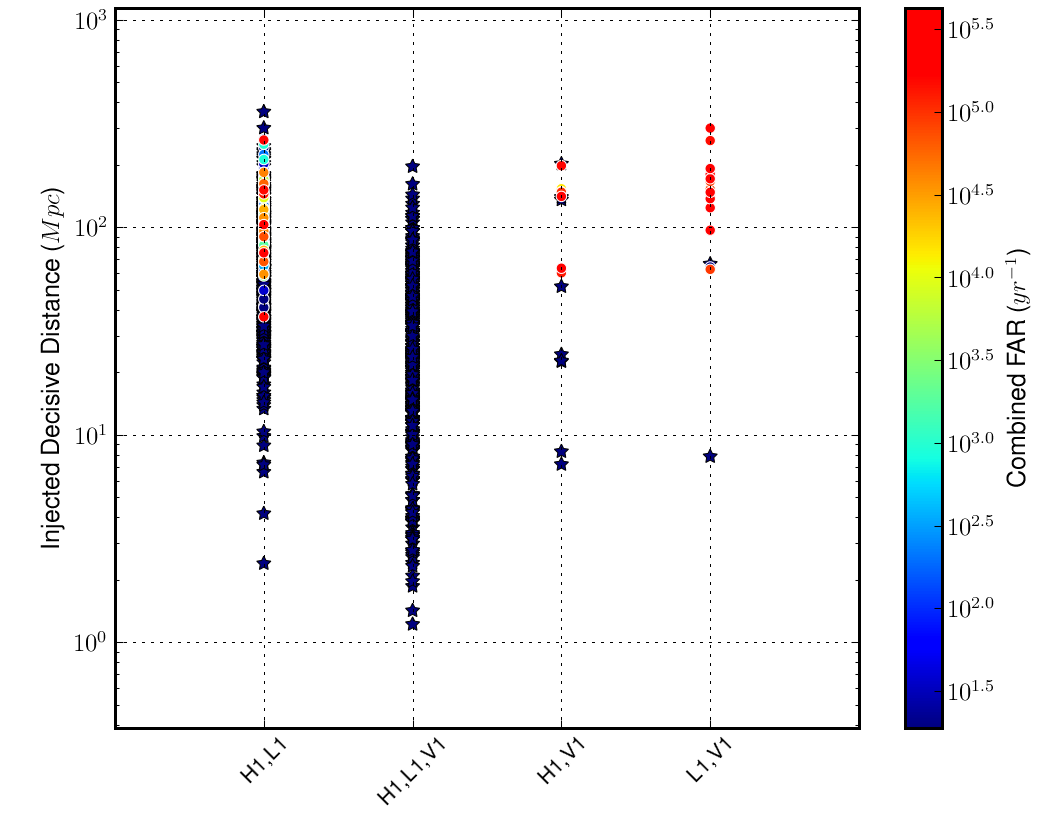
\includegraphics[width=4.8in]{figures/excluding_V1_doubles/plotfm-dist_v_coinc_type-orig.png}}
\subfigure[Recovered chirp mass accuracy v. coincidence type.]{\label{fig:V1doubles-coinc_types-mchirp}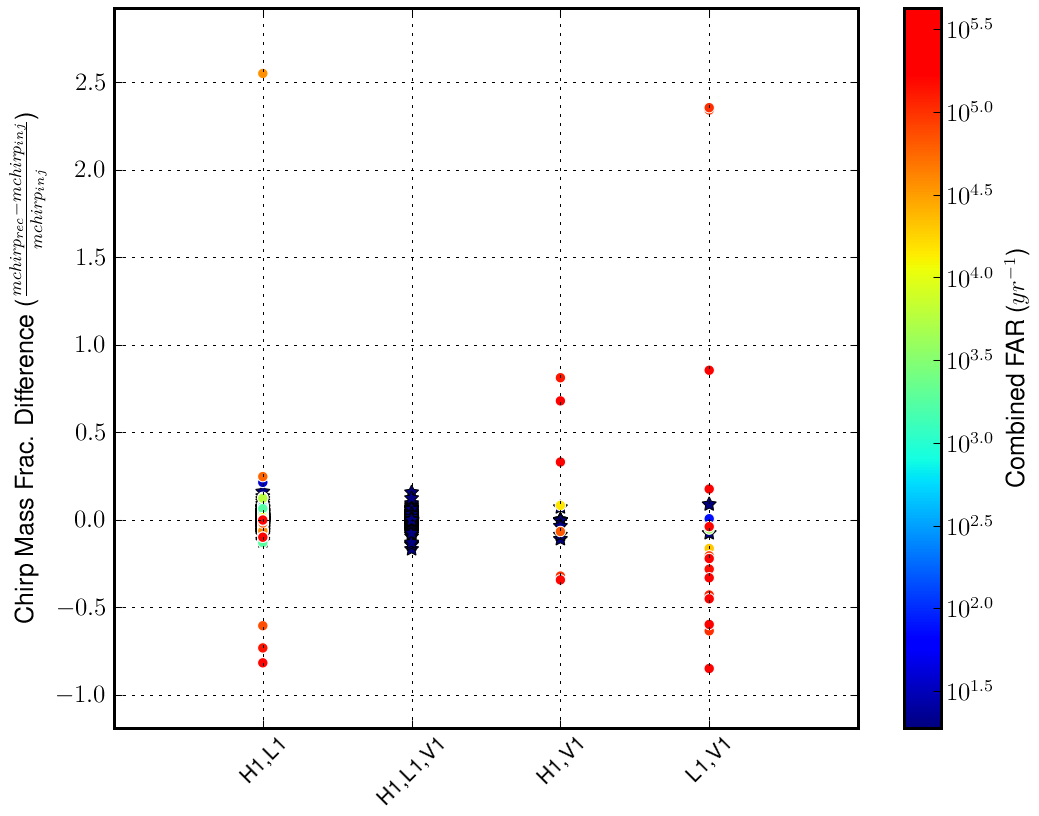
\includegraphics[width=4.8in]{figures/excluding_V1_doubles/plotfm-mchirp_recovery_v_coinc_type-orig.png}}
\label{fig:V1doubles-coinc_types}
\caption{Found injections as a function of the coincidence type that they were
found with. Both plots were created by \texttt{ligolw\_cbc\_plotfm} using the
same data as used in Figure \ref{fig:V1doubles-found_missed}.}
\end{figure}

\begin{figure}[p]
\center
\subfigure[Injections distributed uniformly in linear distance.]{\label{fig:V1doubles-roc-linear}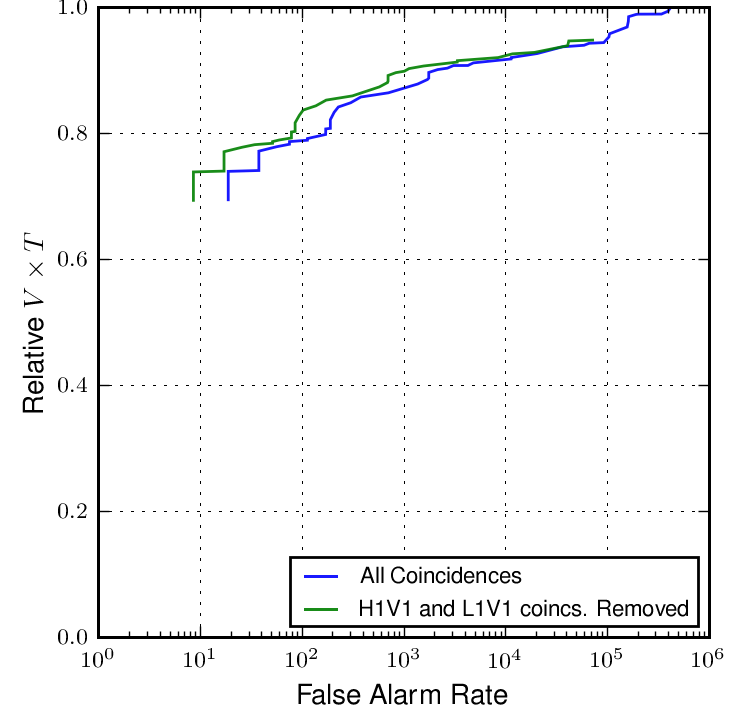
\includegraphics[height=3.5in]{figures/excluding_V1_doubles/lininj_ROC.png}}
\subfigure[Injections distributed uniformly in log distance.]{\label{fig:V1doubles-roc-log}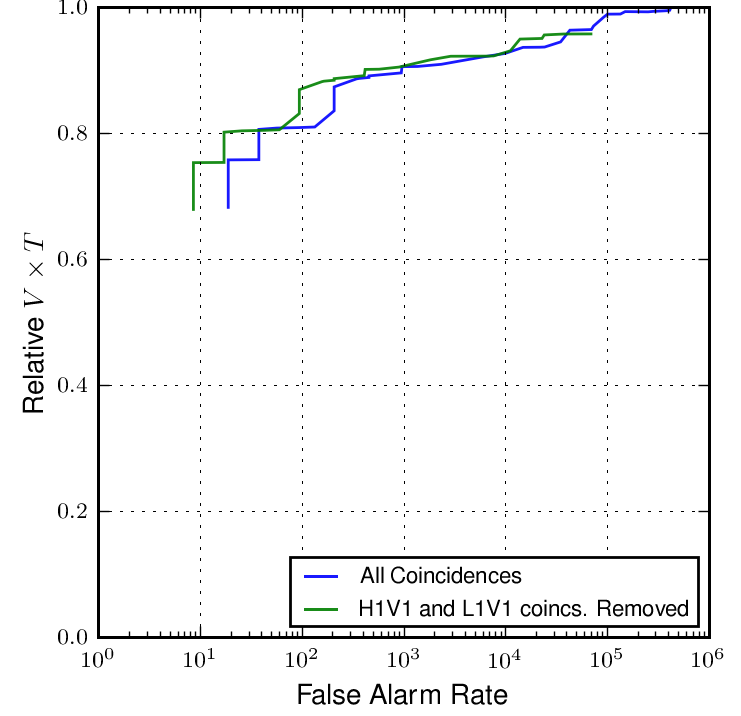
\includegraphics[height=3.5in]{figures/excluding_V1_doubles/loginj_ROC.png}}
\label{fig:V1doubles-roc}
\caption{ROC curves comparing relative sensitive distance in H1L1V1-coincident
time when H1V1- and L1V1-coincident triggers are included (blue curve) to when
they are excluded (green curve). The top plot was created using injections
distributed uniformly in linear distance; in the bottom injections were
distrubted uniformly in log distance. Both plots created by
\texttt{lalapps\_cbc\_plotroc} using the same data as used in Figure
\ref{fig:V1doubles-found_missed}.}
\end{figure}


\section{DQ Issues}
\label{sec:dq_issues}

In the above sections we have described some of the data quality issues that
arose during S6 that resulted in tuning changes. These were the elevated
trigger rate, the switch to a smaller template bank, and the decision to drop
H1V1- and L1V1-coincident triggers in H1L1V1-coincident time during S6D/VSR3.
Here we discuss two of \ac{DQ} issues that we found during \ac{S6} and how we
dealt with them. The two \ac{DQ} topics listed here are by no means exhaustive.
They are simply meant to highlight some results from detailed loudest-slide and
other DQ studies.

\subsection{The H1 \texttt{LVEA\_SEISZ} Veto: An Example Veto using Loudest Slides}
\label{sec:lvea_seismic}

As described in section \ref{sec:s6c}, during S6C and D we used the
loudest-slide triggers from the low-mass \ac{CBC} search to identify potential
new vetoes. Many of the resulting vetoes were only used once based on
observations noted in the e-log of some event at the detector sites. However,
the loudest-slide (i.e., background coincident triggers computed from
time-slides that had the smallest \acp{FAR}) results did result in a few vetoes
that were used extensively. Here we present an example of one of those flags,
the H1 \verb|LVEA_SEISZ| veto.

When we looked at the initial blinded \ihope~page for weeks 13 and 14 of S6C (1
May -- 14 May 2009), we found that the loudest-slide trigger in the high
chirp-mass bin ($\mchirp \geq 7.4\Msun$) had a relatively large combined New
\ac{SNR} of 13.4. The \ihope~analysis of the next two weeks (15 May -- 28 May
2009) also revealed a relatively loud slide trigger, this time in the medium
chirp-mass bin ($3.48 \leq \mchirp/\Msun < 7.4$) with a combined new \ac{SNR} of
11.9. Table \ref{tab:seisz-loud_slides-pre_veto} lists some details about these
triggers. There were no entries in either the Hanford or Livingston e-logs to
suggest a cause for these events. However, as can be seen in Figure
\ref{fig:seisz-loud_slides}, the Omega scans of the H1 \ac{GW} channel showed
similar signatures. When a full-Omega scan was run of every channel at Hanford,
we found considerable seismic noise occuring in the \verb|LVEA_SEISZ| channel
during both events. Figure \ref{fig:seisz-omega_scans} shows the scan from this
channel during these events. The \verb|LVEA_SEISZ| channel monitors vertical
ground motion in the \emph{LVEA}, which is the building that houses all of the
interferometer's central optics, such as the beam splitter, intermediate test
masses, and dark port, as well as the laser.\footnote{The x and y seismic
channels also picked up motion. We used the z channel as it was found to be the
most efficient at targeting resulting glitches in the \ac{GW} channel.}

We therefore developed a flag that monitored the RMS value of the
\verb|LVEA_SEISZ| channel in the $3$--$10\,$Hz band
\cite{detChar:LveaSeiszVeto}. When the channel exceeded 1000 counts (counts are
an arbitrary unit used for \ac{LIGO} channels; they are a measure of the
amplitude of the channel), the flag would go off. Efficiency studies found the
flag to be good at targetting noise transients caused by the seismic noise,
with little ``deadtime" (this is how much time the flag is on for). It was
therefore added as a category-3 veto. Table
\ref{tab:seisz-loud_slides-post_veto} shows the loudest-slide events in the
high and low chirp-mass bin in weeks 13 and 14 and weeks 15 and 16,
respectively, after the application of the veto. The tail of the background
distribution has dropped substantially, and the loudest event is now below a
combined New \ac{SNR} of $11.3$. This means that if a GW signal created a
coincident trigger with a New \ac{SNR} of $8$ in each detector, it would be
louder than all background coincident triggers.

Initially, we only intended to use the flag for weeks 13-16 of S6C. Studies on
the later weeks found that the flag became even more efficient, however, and so
the flag was entered into online monitors as
\verb|H1:DMT-BRMS_SEISMIC_LVEA_Z_3_10_HZ_THRESH_1E3|; it was used as a veto
until the end of S6C. As we had already opened boxes on weeks 1-12, we did not
apply it to those weeks. Further studies showed it would not have been as
effective during those weeks, anyhow. Why this is, and what the cause was for
the increased seismic noise in later weeks of S6C, is unknown
\cite{Lundgren:personal_comm}.

In S6D the \verb|LVEA_SEISZ| veto was superceded by SeisVeto. SeisVeto improved
on \verb|LVEA_SEISZ| by used multiple seismic channels. The output from these
channels were loaded into the hveto algorithm along with daily \ihope~triggers
to find the strongest correlated channels each day. This automation gave even
better efficiency with very little deadtime \cite{detChar:SeisVeto}. For more
details on SeisVeto, see \cite{Macleod:2011}.

\begin{figure}[p]
\center
\subfigure[H1 \ac{GW} channel at 957127982.06 (the loudest-slide event in weeks 13 and 14).]{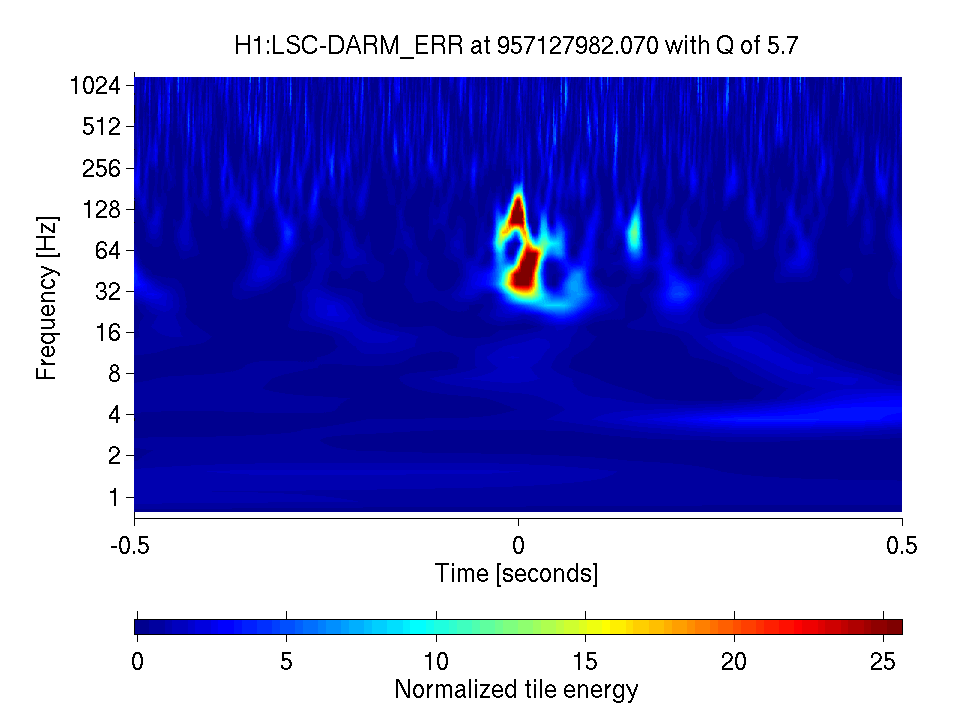
\includegraphics[width=5in]{figures/lvea_seisz-veto/957127982_07_H1-LSC-DARM_ERR_1_00_spectrogram_whitened.png}}
\subfigure[H1 at 958413266.29 (the loudest-slide event in weeks 15 and 16 of S6C).]{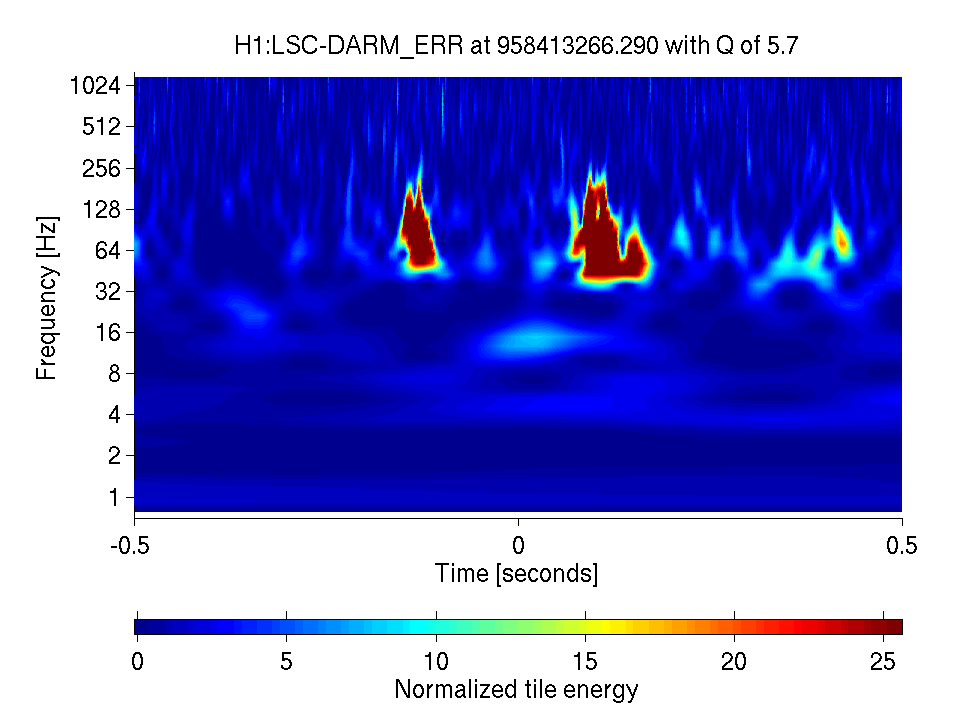
\includegraphics[width=5in]{figures/lvea_seisz-veto/958413266_290_H1_LSC-DARM_ERR_1_00_spectrogram_whitened.png}}
\label{fig:seisz-loud_slides}
\caption{Omega scans of the gravitational-wave channel (\texttt{DARM\_ERR}) during the loudest-slide events shown in Table \ref{tab:seisz-loud_slides-pre_veto}.}
\end{figure}

\begin{figure}[p]
\center
\subfigure[H1 \texttt{LVEA\_SEISZ} at 957127982.06 (the loudest-slide event in weeks 13 and 14).]{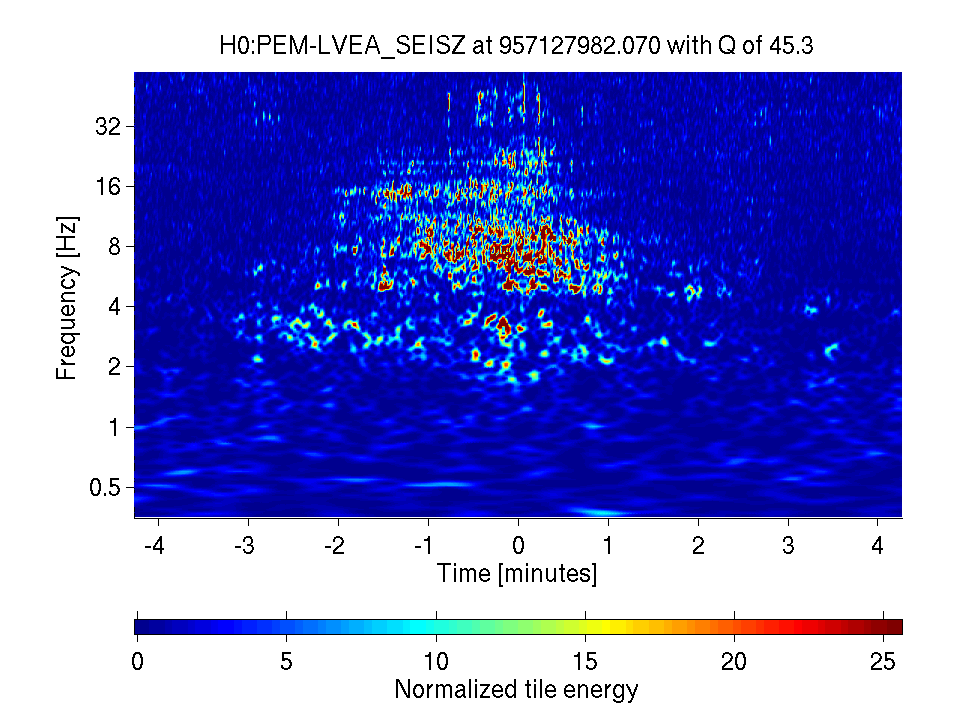
\includegraphics[width=5in]{figures/lvea_seisz-veto/957127982_07_H0-PEM-LVEA_SEISZ_512_00_spectrogram_whitened.png}}
\subfigure[H1 \texttt{LVEA\_SEISZ} at 958413266.29 (the loudest-slide event in weeks 15 and 16 of S6C).]{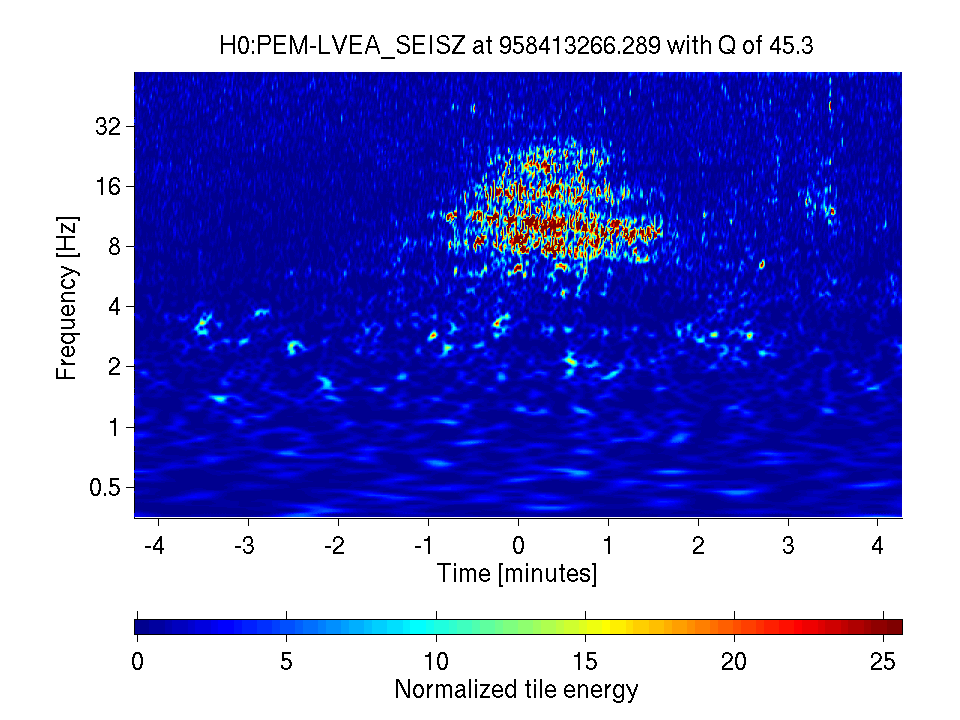
\includegraphics[width=5in]{figures/lvea_seisz-veto/958413266_290_H0_PEM-LVEA_SEISZ_512_00_spectrogram_whitened.png}}
\label{fig:seisz-omega_scans}
\caption{Omega scans of the \texttt{LVEA\_SEISZ} channel during the loudest-slide events shown in Table \ref{tab:seisz-loud_slides-pre_veto}. Note that the time scale is plotted in minutes here whereas in Figure \ref{fig:seisz-loud_slides} it is in seconds.}
\end{figure}

\begin{table}[p]
\center
\begin{small}
\begin{tabular}{| c | c | c | c | c | c | c |}
\hline
\parbox[c]{1.5cm}{Analysis Period}   &   \parbox[c]{1.8cm}{Chirp-mass Bin}   &   $\mchirp (\Msun)$   &   $\mtotal (\Msun)$   &   \parbox[c]{1.8cm}{Combined New \ac{SNR}}   &   \ac{IFO}   &   \parbox[c]{2.5cm}{Single-\ac{IFO} \\End Time \\(GPS seconds)} \\
\hline \hline
\multirow{2}{*}{1 -- 14 May}    &   \multirow{2}{*}{High}    &   \multirow{2}{*}{12.7}   &   \multirow{2}{*}{33.3}    &   \multirow{2}{*}{13.4}    &   H1  &   957127982.06 \\
    &   &   &   &   &   L1  &   957128122.02 \\
\hline
\multirow{2}{*}{15 -- 28 May}   &   \multirow{2}{*}{Medium} &   \multirow{2}{*}{4.0}    &   \multirow{2}{*}{18.8}  &   \multirow{2}{*}{11.9}   &   H1  &   958413266.29 \\
    &   &   &   &   &   L1  &   958413311.36 \\
\hline
\end{tabular}
\end{small}
\caption{The loudest-slide events in the high chirp-mass bin ($\mchirp \geq
7.4\Msun$) of weeks 13 and 14, and in the medium chirp-mass bin ($3.48 \leq
\mchirp/\Msun < 7.4$) of weeks 15 and 16, respectively, of S6C prior to
application of the \texttt{LVEA\_SEISZ} veto. (Being the loudest slide events
in their respective bins, both of these events had 0 combined FAR.) Both
of these events were found to be caused by seismic noise at Hanford.}
\label{tab:seisz-loud_slides-pre_veto}
\end{table}

\begin{table}[p]
\center
\begin{tabular}{| c | c | c | c | c | c | c |}
\hline
\parbox[c]{1.5cm}{Analysis Period}   &   \parbox[c]{1.8cm}{Chirp-mass Bin}   &   $\mchirp (\Msun)$   &   $\mtotal (\Msun)$   &   \parbox[c]{1.8cm}{Combined New \ac{SNR}}   &   \ac{IFO}   &   \parbox[c]{2.6cm}{Single-\ac{IFO} \\End Time \\(GPS seconds)} \\
\hline \hline
\multirow{2}{*}{1 -- 14 May}    &   \multirow{2}{*}{High}    &   \multirow{2}{*}{9.1}   &   \multirow{2}{*}{25.4}   &   \multirow{2}{*}{10.1}    &   H1  &   957858489.74 \\
    &   &   &   &   &   L1  &   957858414.75 \\
\hline
\multirow{2}{*}{15 -- 28 May}   &   \multirow{2}{*}{Medium} &   \multirow{2}{*}{4.4}    &   \multirow{2}{*}{20.9}  &   \multirow{2}{*}{10.3}   &   H1  &   958306864.45 \\
    &   &   &   &   &   L1  &   958306784.5 \\
\hline
\end{tabular}
\caption{The loudest-slide events in the high chirp-mass bin ($\mchirp \geq
7.4\Msun$) in weeks 13 and 14, and in the medium chirp-mass bin ($3.48 \leq
\mchirp/\Msun < 7.4$) in weeks 15 and 16, respectively, of S6C after the
application of the \texttt{LVEA\_SEISZ} veto. (Being the loudest slide events
in their respective bins, both of these events had 0 combined FAR.)}
\label{tab:seisz-loud_slides-post_veto}
\end{table}

\subsection{The ``Spike" Glitch}
\label{sec:spike_glitch}

One of the major \ac{DQ} issues of S6 was the ``Spike" Glitch. Beginning in
August 2009, loud, short-duration ($\sim1\,$ms) glitches began to appear in the
Livingston data. These glitches were characterized by a sharp downward ``spike"
in the \ac{GW} channel followed by ``ringing" (due to the response filters in
the interfermeter); Figure \ref{fig:spike_glitch-closeup} shows a close-up of
one. The glitch would vary in strength; some were so loud that they could be
seen in the raw (unfiltered) time-series of the \ac{GW} channel. Figure
\ref{fig:spike_glitch-example-time_series} shows the time series of an example
loud spike and Figure \ref{fig:spike_glitch-example-omega_scan} shows the
corresponding Omega scan. The high-amplitude noise surrounding the glitch is
due to the impulse response of Omega's whitening filters and the way they
average power over time to highlight transients in the power spectrum.

The spike glitch also adversely affected the \ac{CBC} match filter. Figure
\ref{fig:spike_glitch-cbc_response} shows a typical response by
\verb|lalapps_inspiral| when a spike glitch passes through; in this case the
glitch was the one shown in Figure \ref{fig:spike_glitch-example}. This plot
was created with the $2 \leq \mtotal/\Msun \leq 35$ template-bank, without any
clustering. Each trigger is colored by its $\tau_0$ value, which essentially
gives the duration of the template. The large spike in \ac{SNR} that begins at
the time of the glitch ($0\,$s) is due to the impulse response of the
templates. Although the \ac{SNR} of these triggers is quite large (in this
case, the loudest trigger had a $\rho ~ 8300$), they did not typically show up
in our loudest events nor our loudest slides. This is because they would have
very poor $\chi^2$ values, resulting in low new \acp{SNR}. Of greater concern
was the ``shoulders" surrounding the spike and the tail proceeding the glitch.
This tail could last several seconds after the glitch and its triggers could
have lower $\chi^2$ values. We therefore wished to find the cause of the
glitch, so that the detector could be fixed, or, if that was not possible, so
we could veto it.

\begin{figure}[htb]
\center
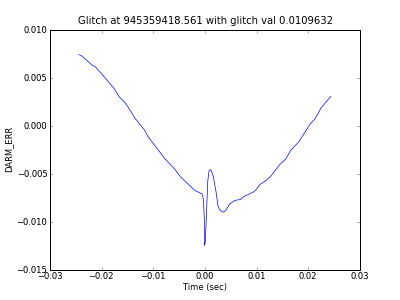
\includegraphics[width=4in]{figures/spike_glitch/spike_glitch_example.png}
\label{fig:spike_glitch-closeup}
\caption{A close-up of a spike glitch. Shown is the \ac{GW} channel (\texttt{DARM\_ERR}) raw time series.}
\end{figure}

Unfortunately, despite a number of intensive data-quality studies and feedback
from instrumentalists, we were never able to determine the cause of the spike
glitch. Not only did this prevent us from fixing the instrument so the glitch
would go away, but it also made it difficult to veto. As stated above, we
typically only veto triggers if they can be strongly correlated with an
auxillarily channel. This is to avoid accidently vetoing a gravitational wave.
The spike glitch was clearly not a \ac{GW}, but we had no other way to veto it
than to use the \ac{GW} channel. We therefore decided to use a DQ flag based on
daily \ihope~triggers. Named \verb|H1:DCH-CBC_SNR_GT_0250|, this flag would go
off whenever triggers exceeded a \ac{SNR} threshold of 250. The flag was used
as a CAT3 veto in S6D, and a ``padding" of $\pm8\,$s was added to it. The
padding was added to remove the ``shoulder" triggers created by the spike.
$8\,$s was chosen based on the length of the inverse spectrum truncation.

There was some concern that vetoing triggers using the output of daily \ihope~
would cause us to miss a nearby event. However, any real GW event that had
a SNR above 250 would stick above the background at CAT2. Since we check
results after CAT2 vetoes have been applied, and the SNR $> 250$ flag was
applied at CAT3, this veto would not prevent us from detecting such an event.

\begin{figure}[hp]
\center
\subfigure[Raw time series.]{\label{fig:spike_glitch-example-time_series}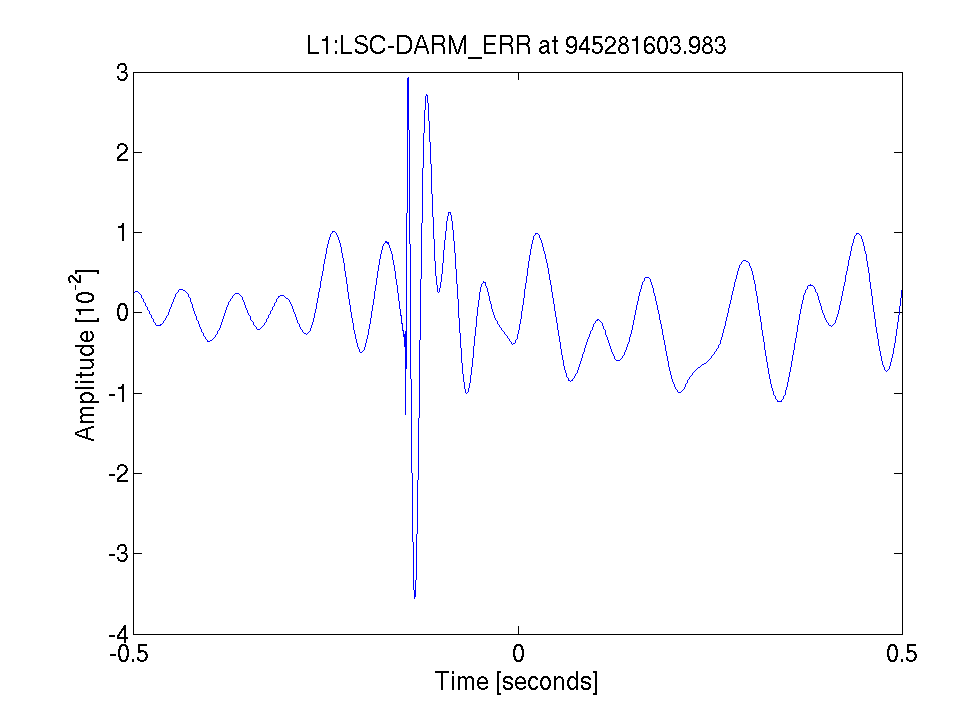
\includegraphics[width=4in]{figures/spike_glitch/945281603_spike_glitch-raw_time_series.png}}
\subfigure[Omega scan.]{\label{fig:spike_glitch-example-omega_scan}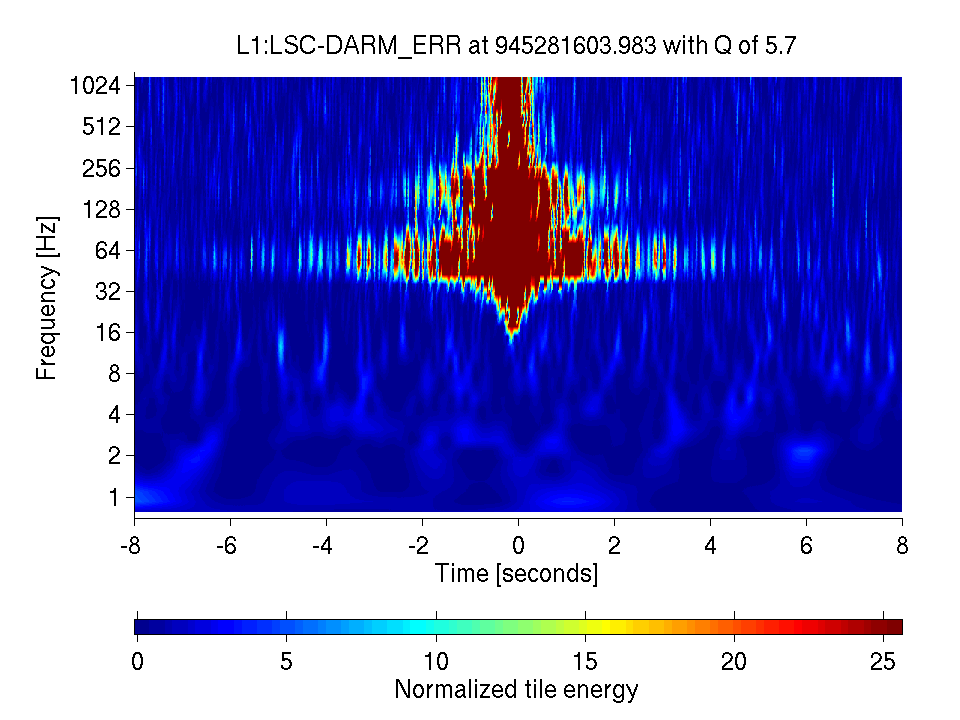
\includegraphics[width=4in]{figures/spike_glitch/945281603_9826171875_L1-LSC-DARM_ERR_16_00_spectrogram_whitened.png}}
\label{fig:spike_glitch-example}
\caption{An example spike glitch. This glitch occurred at GPS time 945281603.98
(19 December 2009 18:13:08 UTC). The top plot shows the raw time series from
the GW channel; no filtering has been applied to this plot. The bottom plot
shows the Omega scan of this glitch. Omega uses a whitening filter to create
the bottom plot, hence the high-ampltiude noise lasts several seconds.}
\end{figure}

\begin{figure}[hp]
\center
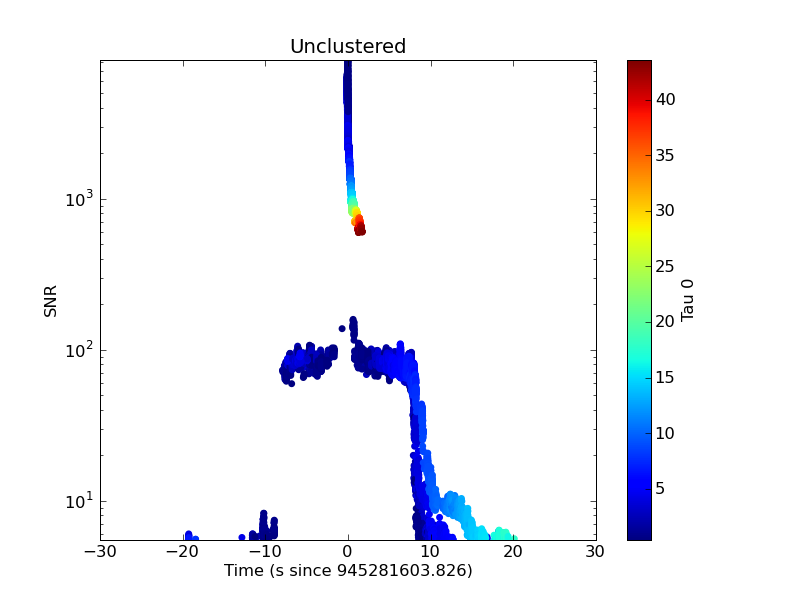
\includegraphics[width=4in]{figures/spike_glitch/L1_945281603.png}
\label{fig:spike_glitch-cbc_response}
\caption{The unclustered triggers created by the spike glitch shown in
\ref{fig:spike_glitch-example} when passed through \texttt{lalapps\_inspiral}.}
\end{figure}

\section{Results}

As described in section \ref{sec:s6_epochs}, we initially analyzed the data in
several small analysis periods --- weekly runs in S6a; three month-long chunks
in S6B; bi-weekly runs in S6C and D --- and opened boxes on each of these
analyses. We did this so we could obtain results quickly, and so we could
pro-actively adapt the pipeline to \ac{DQ} issues, as detailed above. However,
we did this with the knowledge that we would have to re-run the pipeline over
these periods. Re-runs were required in order to take advantage of final
calibration studies, as well as fix minor issues in published veto
segments.\footnote{Upon review, a CAT1 veto-flag was found to stay on (and off)
for slightly longer periods than it should have. The effect on the analysis is
small, amounting to a change in livetime of less-than a day across all of S6.
For the sake of rigor, however, we have fixed the flag for re-runs.} For speed
and simplicity these re-runs are being carried out in larger $\sim6$-week long
chunks.  S6A is being analyzed with one run; S6B is divided into two chunks,
one prior to 11 November 2009, and the other from 11 November to 11 January
2010. S6C and D are each being re-analyzed in three chunks. Aside from the
grouping of analysis periods together, no other changes have been made to the
runs. For example, although new vetoes were created throughout S6C and D, these
have not been retroactively applied to earlier periods.

As the changes between the original runs and the final re-runs are minor, we do
not expect our result to change. The result of the S6/VSR2/3 analysis is: No
gravitational-wave candidates were detected. Currently, the most significant
event is an H1L1-coincident trigger in H1L1V1-coincident time with a combined
FAR of \firstFAR. The second and third most significant triggers had combined
FARs of \secondFAR~and \thirdFAR, respectively. All of these triggers are
consistent with background: having analyzed $\mathrm{\sim0.5~yr}$~of data, we
would expect the loudest event to have a FAR of \expectedLoudestFAR. Although
no detection candidates have been found, we will perform detailed follow-ups on
the loudest triggers in each epoch once the re-runs have completed. These
followups are carried out to aid in future \ac{DQ} investigations.

As a part of the re-runs we are performing extra injection runs. This is so we
can improve our statistics for placing upper-limits. Since these runs are still
on-going, and since the final upper limits will need to be reviewed once they
are produced, we do not present upper limits here.

\section{The Blind Injection}
\label{sec:s6_results_and_big_dog}

A hardware injection was injected into the \ac{LIGO} and Virgo detectors during
S6D/VSR3 without the search groups' knowledge.\footnote{The search groups did
know that zero or more blind injections could happen over the course of
the Science run, however.} The purpose of this \emph{blind-injection challenge}
was to test the groups' abilities to detect signals and to exercise the LIGO
and Virgo Collaborations' procedures in the event that a real
gravitational-wave candidate is detected. The {\it blind injection} was found
by the \ac{CBC} group with a FAR low enough to be considered a detection
candidate. We treated the event as if it were real: detailed studies were done
to establish the significance and parameters of the event, and to vet the
detectors of any possible environmental or instrumental causes. Only after all
procedures were reviewed and a paper draft written was the event unveiled as an
injection.  Although the event was not real, we present here details of the
analysis of the injection, including methods used to calculate its \ac{FAR}.

\subsection{Observation and FAR Estimation}

The blind injection occurred on \dogDate~at \injectedDogTime~(GPS time
\injectedDogGPSTime) and was identified by multiple searches. It was initially
observed, within a few hours, by a low-latency Burst search. Since Burst
searches use un-modelled waveforms, it did not give the event a \ac{FAR} small
enough to be considered a detection. However, it was signifcant enough to stand
out as a potential \ac{CBC} candidate, and so the collaboration was alerted to
its prescence in the data.

Although we knew about the potential candidate prior to opening the box, we
carried out the analysis of the two weeks containing the event as we did every
other period: a blinded \ihope~page was generated, loudest-slides were
examined, vetoes were updated, and a re-run was carried out with the new vetoes
to prepare of the unblinding of the results. The injection was loud enough in
H1 that it was a part of the loudest H1L1-slide event in the medium chirp-mass
bin during H1L1V1-coincident time. In this event the candidate in H1 was
coincident with a random noise event in L1. The slide event had a combined New
\ac{SNR} of 11.56 and the chirp was visible in the H1 Omega scan. (See Table
\ref{tab:big_dog-loudest_slides} for more details.) As with any loud
slide-event we checked the \ac{DQ} studies for the week and the e-log to see if
we could find an auxillarily channel to veto the times in either of the
detectors.\footnote{Since the blind injection is a hardware injection, it is
created by actuating one of the mirrors. There is a channel that monitors the
input to this mirror, and so it is possible to check whether or not an event is
a blind injection without having to wait for the ``envelope" to be opened. We
forbid ourselves from checking this channel, however, as it would make the
entire challenge pointless.} No cause could be found in either detector, and so
the slide event stayed in the data.

When the box was opened the injection was found as \emph{two} events: one in
the low chirp-mass bin, and one in the medium chirp-mass bin. Both triggers
were found as H1L1 coincidences in H1L1V1 time and had combined \acp{FAR} of
zero; i.e., both events were louder than all the background in their respective
bins. Figure \ref{fig:big_dog-ifar} shows the unblinded IFAR plot for
H1L1V1-coincident time from the analysis and Table
\ref{tab:big_dog-loudest_events} shows the parameters of the two events that
were found. That the injection created two triggers was a result of our earlier
decision to cluster coincident triggers within each chirp-mass bin. Since both
triggers had zero combined \acp{FAR} it was not immediately clear which trigger
to keep. Further complicating the matter was that the triggers landed exactly
on the bin boundary: the low-mass trigger had a chirp mass of $3.47\,\Msun$ and
the high mass trigger had a chirp mass of $3.48\,\Msun$; the boundary was
$\mchirp = 3.48\,\Msun$. Since we needed to estimate a combined \ac{FAR} for
the candidate, we decided to find an estimate in each bin. Whichever trigger had
the lower-combined \ac{FAR} we would keep.

In order to estimate a \ac{FAR} for the candidate event we initially combined
data from adjacent analysis periods. This was standard procedure; it was performed
on several different occasions in prior instances when a trigger was found with
zero \ac{FAR} in a single week of analysis. However, the candidate was the loudest
H1L1-coincident trigger in all of S6. Thus, even if we used all the data in S6, we could
still only estimate the \emph{uncombined} \ac{FAR} to be $< 1$ in $23$ years.
This was not small enough to claim a detection. It was also not clear that
using data from all of S6 was the correct approach, since the data quality had
changed substantially from S6A to when the event occurred, in S6D.
Additionally, computing a combined \ac{FAR} using data from across epochs would
have been difficult, since in S6A and B the trials factor in H1L1V1 time was
12, in S6D it was 6, and in S6C there was only H1L1 time. 

To get a better estimate of the \ac{FAR}, two methods were pursued. One was to
perform an extrapolation using data from the 100 slides. Figure
\ref{fig:big_dog-non_cum_hist-extrap} shows a histogram of all of the H1L1
triggers in S6C and D as a function of combined new \ac{SNR} ($\rhonewc$) in
the low and medium chirp-mass bins. Zero-lag triggers are represented as blue
dots; slide triggers are black. The blind injection is the blue dot all the way
to the right, at $\rhonewc \approx 12$. The structure of the distribution is
largely due to $\chi^2$ re-weighting and the \ac{SNR} cutoff: non-Gaussian
triggers have been down-weighted, removing any tail in the distribution, and
the peak at $\rho_{nc} \approx 8$ is due to the \ac{SNR} cut. Indeed, any
trigger below a combined new \ac{SNR} of 7.7 ($= \sqrt{2}\times 5.5$) must be a
trigger that was down-weighted, since we apply the \ac{SNR} cut at 5.5. For
combined new \acp{SNR} $> 8.5$ the distribution appeared to be Gaussian,
particularily in the low chirp-mass bin. We therefore performed a least-squares
fit to the background distribution using a Gaussian of the form:
\begin{equation*}
A exp\left[ -\frac{x^2}{2\pi\sigma^2} \right]
\end{equation*}
where $A$ and $\sigma^2$ were the fit parameters. We used the slide data in the
range $\rhonewc \in [8.5, \max(\rhonewc)]$ to peform the fit. The green-dashed
line shows the result of the fit.

Next, we created a cumulative histogram plot in each bin, shown in Figure
\ref{fig:big_dog-cum_hist-extrap}, with the y-axis normalized by the zero-lag
live time. Using the fitted parameters from the non-cumulative histograms, we
plotted the complimentary error function:
\begin{equation*}
y(\rhonewc) = A\mathrm{erfc}\left(\frac{\rhonewc}{\sqrt{2\sigma^2}}\right)
\end{equation*}
This is shown as the green-dashed line, from $\rhonewc = 8.5$ to the combined
New \ac{SNR} of the blind injection. Thus, the point on the y-axis where the
green-dashed line ends gives the uncombined \ac{FAR} of the blind injection. In
the low chirp-mass bin this yielded a \ac{FAR} $\approx 1$ in $4\times 10^{6}$
years, and in the medium bin we obtained a \ac{FAR} $\approx 1$ in $2\times
10^{6}$ years.

On the cumulative histogram plots we additionally plotted the probability
density function that the zero-lag events came from the background distribution
as a color map. This map was computed using the Poisson distribution (equation
\ref{eqn:poisson} in Chapter \ref{ch:far}). At each point along the x-axis,
$\lambda$ was determined using the cumulative rate of the closest slide data
point greater-than that point. For points past the loudest-slide point
(indicated by the vertical black line), the extrapolation is used. Note that
this was done prior to dividing by the zero-lag live time, so that the
cumulative-rates were unitless; i.e.:
\begin{equation*}
\lambda = N_{\mathrm{cum,slide}} \frac{T_{\mathrm{f}}}{T_{\mathrm{b}}}
\end{equation*}
where $N_{\mathrm{cum,slide}}$ is the number of slide triggers with $\rhonewc
\geq$ the combined new \ac{SNR} at the given point on the x-axis,
$T_{\mathrm{f}}$ is the zero-lag live time, and $T_{\mathrm{b}}$ is the total
slide live time. The probablity density at each point along the y-axis at that
x-value is then determined by substituting the (unitless) y-value as $k$ in
equation \ref{eqn:poisson}. The entire plot was then divided by $T_{\mathrm{f}}$ to
get it into units of yr$^{-1}$. The color map ends at $y = 1 / T_{\mathrm{f}}$
because the Poisson distribution is not defined for $k < 1$. (Technically, it
is not defined for any non-integer $k$. To make the plot cleaner we
interpolated between integer points using the Gamma Function.) The black
dashed-lines indicate $N\sigma$ points, as determined by the Gaussian
distribution. For example, $2\sigma$ corresponds to a probabliity density of
$0.045$, and so the second black dashed-line maps out points where the
distribution is equal to $0.045$. We do this because a false alarm probability
equal to $5\sigma$ is generally considered the ``gold" standard for a new
detection in the particle physics community.

While the extrapolation appears to fit the low chirp-mass bin well, it clearly
deviates from the slide distribution in medium chirp-mass bin. This is largely
due to the loudest slide event, which happens to be the event shown in the
first row of table \ref{tab:big_dog-loudest_slides}: it resulted from the blind
injection in H1 being coincident with a random noise event in L1. If we remove
$\pm8\,s$ around the end time of the injection from each detector when
performing the slides, then any slide event that could be caused by the blind
injection goes away. Figure \ref{fig:big_dog-cum_hist_no_littles-extrap} shows
the cumulative histogram for the low and medium chirp-mass bins when this is
done. The low chirp-mass bin is largely unaffected, but in the medium mass bin
the fit matches better. The extrapolated \acp{FAR} were largely unaffected when
doing this; both low and medium chirp-mass bins still gave $\approx 1$ in
$4\times 10^{6}\yr$ and $\approx 1$ in $2\times 10^{6}\yr$, respectively.

We did not feel confident using these extrapolated \acp{FAR}. The validity of
extrapolating over six orders of magnitude was hard to determine. Additionally,
we had no expected model for the background. Even if new \ac{SNR} removed all
non-Gaussian transients above an \ac{SNR} of 5.5 we had no model for the
effects of coincidence testing and the various stages of clustering. We chose
to fit a Gaussian largely because that is what the slide distribution looked
like. However, even when the blind injection was excluded from the background
estimation, the extrapolation still appeared to deviate slightly from the slide
triggers in the medium chirp-mass bin. This suggested that a Gaussian was not
the correct distribution to use in the medium bin.

The 100 slides that we typically do is a small percentage of the total number
of possible slides. Thus, another way to estimate the \ac{FAR} was to do more
time slides. Since we use offsets that are multiples of $5\,$s between H1 and
L1 in the standard search, we decided to do the maximum number of $5\,$s slides
that was possible in S6D. We limited the estimation to S6D to try to ensure
that the background rate was roughly constant across the period (recall from
Chapter \ref{ch:far} that assumming a stationary source is central to the
\ac{FAR} analysis). Also, rather than perform slides on rings, we used linear
slides.\footnote{Recall from section \ref{sec:second_thinca} that
\texttt{lalapps\_thinca} slides single-detector triggers on \emph{rings} prior
to doing the coincidence test. Triggers that are slid past the end time of the
a particular file are placed at the beginning. Since \texttt{thinca} jobs are
set-up so that only span coincident detector times (after CAT1 vetoes have been
applied), any times for which a single detector is operating (``single-detector
time") will not be used for the coincidence test. Contrast this to \emph{linear
slides}, in which triggers are slid without regard to when a particular
\texttt{thinca} file starts or ends. Thus, single-detector times can be slid
into coincident-detector time.} This way we could use single-detector times in
the background estimation. In this manner we were able to perform $~4\times
10^6$ slides, resulting in $\sim 1 \times 10^6$ \emph{effective slides}.
(Recall from chapter \ref{ch:far} that the effective slide number is obtained
by dividing the total slide live time by the zero-lag live time.) This resulted
in a total background live time of $2.0\times 10^5$ years. To remove any effect
on the background estimation from the first coincidence testing, we created a
list of single-\ac{IFO} triggers with $\chi^2$ values using a proto-type
single-stage pipeline. This pipeline was the same as the \ac{HIPE} pipeline
described in Chapter \ref{ch:ihope_pipeline}, except that $\chi^2$ was
calculated at first Inspiral and no second stage was carried out. 

Two independent scripts were used to carry out the slides to check the results.
Due to the computational cost of doing so many slides, only single-\ac{IFO}
triggers that had new \acp{SNR} large enough to cause a coincidence as loud or
louder than the injection's combined new \ac{SNR} were considered by both
scripts. Additionally, since the injection was found as an H1L1 event, we did
not use V1 in the analysis. Thus we effectively combined H1L1V1 time and H1L1
time into one, and pulled out all H1L1 coincidences from potential H1L1V1
triggers. Both scripts agreed with each other. The result was that there were
$4$ coincidences with combined new \acp{SNR} $\geq$ the injection's $\rhonewc$
in the low chirp-mass bin, giving an uncombined \ac{FAR} of $1$ in $50,000$
years. In the medium chirp-mass bin there were $5$ louder coincidences, giving
an uncombined \ac{FAR} of $1$ in $40,000$ years. This was with the candidate
event left in the background. If the candidate was removed, no coincidences
were louder than it, putting a limit on the uncombined \ac{FAR} of $< 1$ in
$200,000$ years. One of the two scripts was able to additionally compute the
\ac{FAR} using $1$ second slides. When this was done, one event was found to be
louder than the injection even when it were removed in the low chirp-mass bin.
In the middle chirp-mass bin, however, there were still no events louder than
the injection. Based on this result, along with the fact that the combined new
\ac{SNR} was larger in the middle chirp-mass bin, we decided to keep the
trigger in the middle bin, i.e., the one with a chirp mass of $3.48\Msun$, and
discard the other.

Figure \ref{fig:big_dog-rate_plot} summarizes these results, which is a
cumulative histogram in the middle chirp-mass bin. This plot was created in the
same manner as the cumulative plots shown in Figures
\ref{fig:big_dog-cum_hist-extrap} and (minus the extrapolation). Here, the
zero-lag triggers in S6D (S6C is not included) are the blue triangles. The
background from the standard 100-slide analysis are represented by the dots.
The crosses represent the loudest triggers from the $4$ million $5$ second
slides. The black dots and crosses are from the background estimations in which
the injection was left in the background. The gray dots and crosses are from
the background estimation if the injection is excluded. Rather than use a color
map to show the probability density, we plotted shaded contours to represent
the $1$--$5\,\sigma$ regions of the \ac{PDF}. The contours were calculated
using the background with the injection left in. Had the injection been a real
event, this plot would have been our main figure of merit in the resulting
detection paper.

The question of whether or not to leave the injection in the background was
hotly debated prior to opening the envelope. If the event were a real
gravitaional-wave, we would remove it from the data. Otherwise, leaving it in
would break the assumption, made at the end of Chapter \ref{ch:far}, that the
total rate density calculated from time-slides is the same as the \ac{FAR}. In
this case the noise/GW terms in equation \ref{eqn:eqn:slideTerms} at low
\ac{FAR} would be on par with the noise/noise term. Thus we could not make the
approximation in equation \ref{eqn:eqn:valid_slide_condition}. Yet if the event
were from noise, removing it would underestimate its \ac{FAR}, as well as the
\ac{FAR} of all other events. Ultimately we decided to present both backgrounds
on the plot (and in the detection paper), but, to be conservative, quote the
false alarm rate with the event left in the background. (This is why the
background points with the injection left in are black, whereas the event-free
background points are light gray, and why the probability contours are based on
the former estimate.) Thus the quoted uncombined false alarm rate for the event
was $1$ in $40,000$ years.

To get a combined \ac{FAR} for the injection we multiplied the uncombined
\ac{FAR} by a trials factor of 6. This gave a final false alarm rate for the
event of $\sim1$ in $7000$ years. Since we folded all H1L1 triggers in
together, this was a slight overestimate. Had we included V1, some of those
triggers would have been H1L1V1 coincidences, and so would have been excluded
from the bin. Determining what triggers would have formed triple-coincidences
would have been impossible because we folded H1L1 time together with H1L1V1
time. While we could have determined what triggers would have been coincident
with V1 in H1L1V1 time, we could not know this in H1L1 time. Since the number
of H1L1V1 coincidences are typically small compared to the number of H1L1
triggers, however, this overestmiate would have been minor.

Even with the injection left in the background, the event was still close
to a $5\sigma$ event, as can be seen in \ref{fig:big_dog-rate_plot}. Thus we
went a head with writing a detection paper, and a number of intensive
data-quality investigations were carried out on the period of time. The event
passed all tests.  The LIGO observatories were in quiet night-time operation
with near maximum astrophysical range; the Virgo detector had quiet
environmental conditions, except for elevated micro-seismic levels. The lack of
an observed signal in Virgo was consistent with a \ac{GW}. V1's sensitivity was
a factor of four lower than the LIGO detectors at the time. Since the largest
single-\ac{IFO} \ac{SNR}, recorded in H1, for the event was $\sim15$ (note the
H1 \ac{SNR} in the loudest slides in table \ref{tab:big_dog-loudest_slides}),
it very likely had a \ac{SNR} below our threshold of $5.5$ in V1.

\subsection{Conclusions}

The blind injection challenge in S6 was considered a success. The event was
identified, a false alarm rate was calculated, and it was vetted by \ac{DQ}
investigations. For the first time we wrote a paper detailing a highly-probable
\ac{GW} detection. Had the event been real this paper would have been
published. Even though it was not real, the experience gained will prove
valuable for the first real detection, which is expected to happen in  advanced
LIGO. In addition to highlighting the strengths of our pipeline, it also
unearthed some weaknesses. That a \ac{GW} event can hurt its own \ac{FAR} if
left in the background estimation was not fully appreciated prior to the
exercise. How exactly to deal with this scenario, particularily if there are
multiple \acp{GW} in the data, is still an open question. It will be an area of
active research between now and advanced LIGO.

After the event was revealed to be a blind injection, a veto was created for it
and it was removed from the data. As stated above, with the injection removed,
there were no gravitational-wave candidates in S6/VSR2/3. A paper presenting
updated upper-limits as well as more details about the blind injection is in
progress.

\begin{figure}[p]
\center
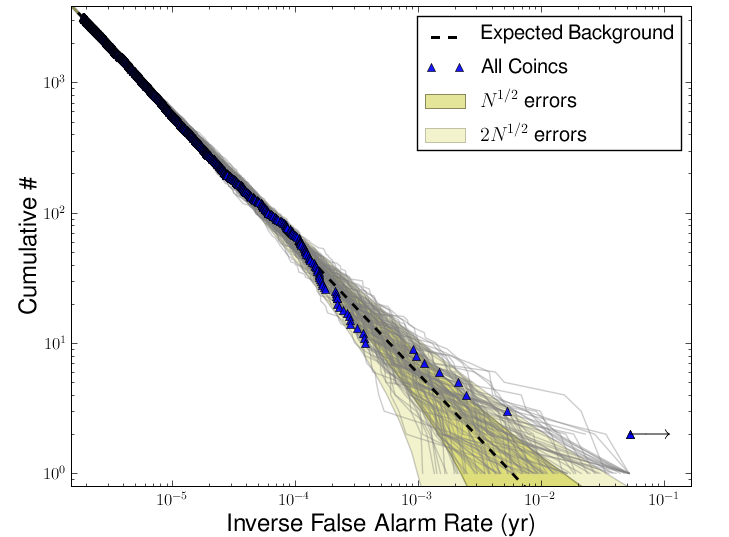
\includegraphics[width=6in]{figures/big_dog/H1L1V1-ligolw_cbc_plotifar_FULL_DATA_CAT_4_VETO_cumhist_combined_ifar_ALL_DATA_PLOTTED_OPEN_BOX-967593543-1209744.png}
\caption{IFAR plot from the two-week-long \ihope~run containing the blind
injection. The two coincident triggers that the injection created can be seen
as the triangle with a cumulative number of 2 at the lower-right of the plot.
Note the arrow pointing to the right. This indicates that the two triggers were
louder than all slide-coincident triggers in the two-week long analysis period
that the injection occurred in.}
\label{fig:big_dog-ifar}
\end{figure}

\begin{table}[p]
\center
\begin{small}
\begin{tabular}{| c | c | c | c | c | c | c | c |}
\hline
\parbox[c]{1.8cm}{Chirp-mass Bin}   &   \parbox[c]{1.8cm}{Combined New \ac{SNR}}   &   \parbox{1cm}{$\mchirp$\\$(\Msun)$}   &   \parbox{1cm}{$\mtotal$\\$(\Msun)$}   &   \ac{IFO}   &   \parbox[c]{1.9cm}{Single-\ac{IFO} \\New \ac{SNR}}    &   \parbox[c]{1.9cm}{Single-\ac{IFO} \\ \ac{SNR}}    &   \parbox[c]{1.8cm}{Effective \\Distance (Mpc)} \\
\hline \hline
\multirow{2}{*}{Low}    &   \multirow{2}{*}{12.06}   &   \multirow{2}{*}{3.47}    &   \multirow{2}{*}{24.01}   &   H1  &   10.29   &   12.14   &   54.6 \\
    &   &   &   &   L1  &   6.29    &   8.25    &   83.6    \\
\hline
\multirow{2}{*}{Medium} &   \multirow{2}{*}{12.48}   &   \multirow{2}{*}{3.48}  &   \multirow{2}{*}{23.17}   &   H1 &   10.29   &   12.14   &   54.6    \\
    &   &   &   &   L1  &   7.06    &   8.854   &   81.2 \\
\hline
\end{tabular}
\end{small}
\caption{The two events resulting from the blind injection that survived
clustering. Both events occured at GPS time $968654557.87$, and had a zero
combined FAR.}
\label{tab:big_dog-loudest_events}
\end{table}

\begin{table}[p]
\center
\begin{small}
\begin{tabular}{| c | c | c | c | c | c | c | c |}
\hline
\parbox[c]{1.5cm}{Analysis} &   \parbox[c]{1.8cm}{Combined New \ac{SNR}}   &   \parbox{1cm}{$\mchirp$\\$(\Msun)$}   &   \parbox{1cm}{$\mtotal$\\$(\Msun)$}   &   \ac{IFO}   &   \parbox[c]{1.9cm}{Single-\ac{IFO} \\New \ac{SNR}}    &   \parbox[c]{1.9cm}{Single-\ac{IFO} \\ \ac{SNR}}   &   \parbox[c]{2.5cm}{Single-\ac{IFO}\\End Time\\($968654558 + $s)} \\
\hline \hline
\multirow{2}{*}{\parbox[c]{1.5cm}{100\\slides}} &   \multirow{2}{*}{11.56}    &   \multirow{2}{*}{4.62}    &   \multirow{2}{*}{13.41}   &   H1   &   10.33    &   15.34   &   0   \\
    &   &   &   &   L1    &   5.19    &   5.64    &     $-230$ \\
\hline
\multirow{2}{*}{\parbox[c]{1.5cm}{$4\times10^{6}$\\$5\,$s slides}}  &   \multirow{2}{*}{12.67}  &   \multirow{2}{*}{4.40}   &   \multirow{2}{*}{16.53}  &   H1  &   10.33   &   15.34   &   0   \\
    &   &   &   &   L1  &   7.33    &   8.48   &   $-5548535$   \\
\hline
\end{tabular}
\end{small}
\caption{The loudest slide events in the medium chirp-mass bin involving the
blind injection in the standard, 100 slide analysis, and in the $4\times10^{6}$
$5\,$s slide analysis. In both cases the injection in H1 is coincident with
noise in L1.}
\label{tab:big_dog-loudest_slides}
\end{table}

\begin{figure}[p]
\center
\subfigure[H1]{\label{fig:big_dog-omega_scans-H1}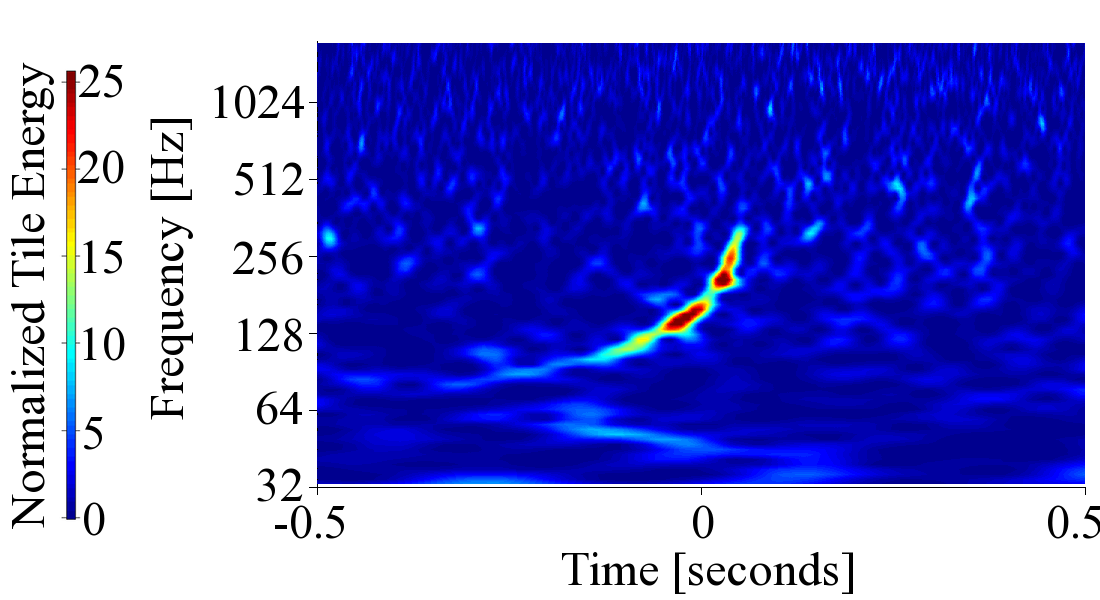
\includegraphics[height=1.75in]{figures/big_dog/omegagram_h1.png}}
\subfigure[L1]{\label{fig:big_dog-omega_scans-L1}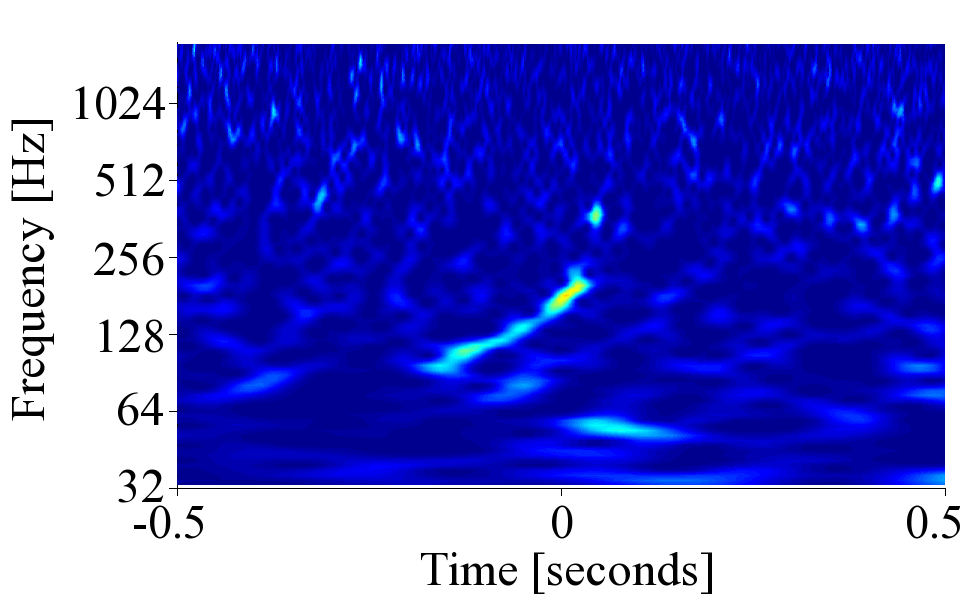
\includegraphics[height=1.75in]{figures/big_dog/omegagram_l1.png}}
\subfigure[V1]{\label{fig:big_dog-omega_scans-V1}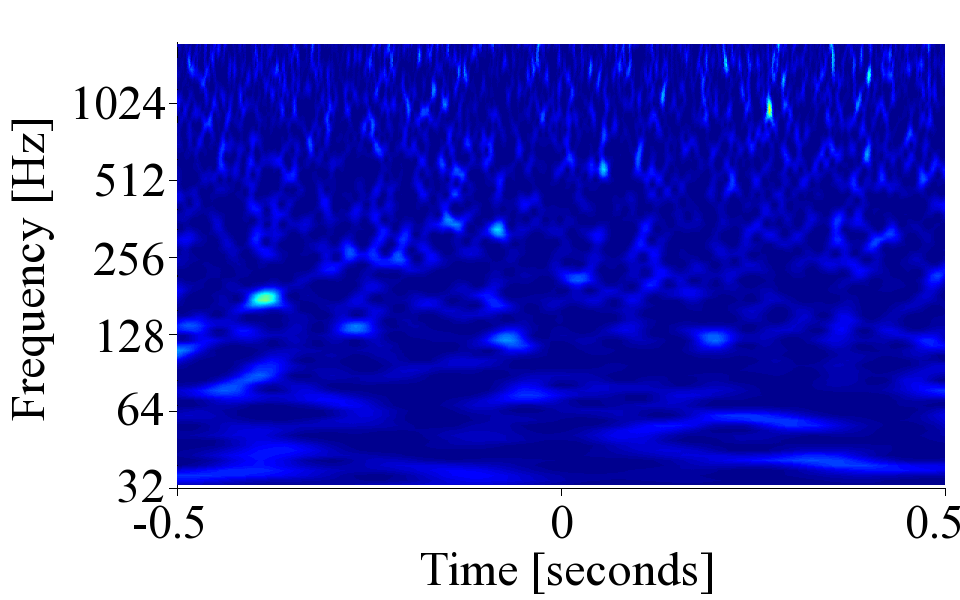
\includegraphics[height=1.75in]{figures/big_dog/omegagram_v1.png}}
\caption{Omega scans of H1, L1, and V1 at the time of the blind injection. The chirp is clearly visisble in H1 and L1.}
\label{fig:big_dog-omega_scans}
\end{figure}

\begin{figure}[p]
\center
\subfigure[The low chirp-mass bin.]{\label{fig:big_dog-non_cum_hist-extrap_low}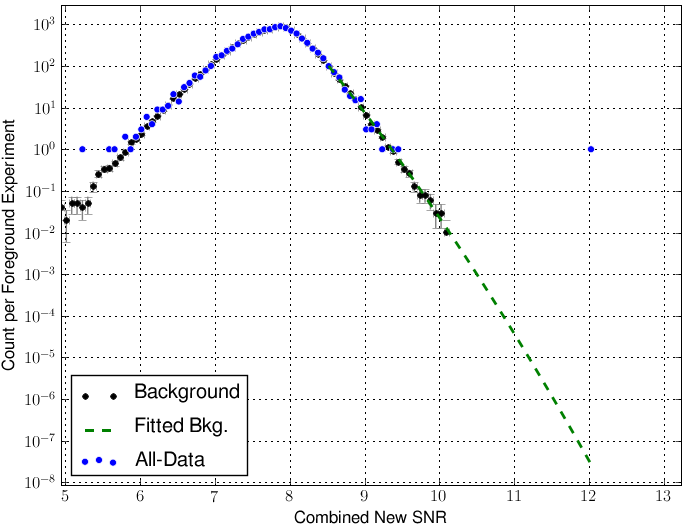
\includegraphics[height=3in]{figures/big_dog/plotrates-non_cum_hist_ext-low_mchirp_bin-S6CD.png}}
\subfigure[The medium chirp-mass bin.]{\label{fig:big_dog-non_cum_hist-extrap_med}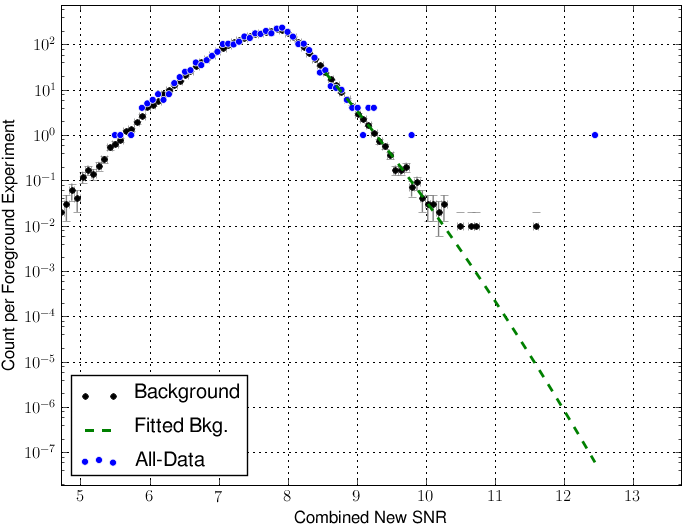
\includegraphics[height=3in]{figures/big_dog/plotrates-non_cum_hist_ext-med_mchirp_bin-S6CD.png}}
\caption{Histograms of all of the H1L1 triggers in S6C and D as a function of
combined New SNR ($\rhonewc$) in the low and medium chirp-mass bins. Zero-lag
triggers are represented as blue dots; slide triggers are black. The y axes are
normalized by $T_{\mathrm{exp}}/T_{\mathrm{f}}$, where $T_{\mathrm{exp}}$ is
the duration of the experiment type for a given set of points --- zero-lag or
slide --- and $T_{\mathrm{f}}$ is the zero-lag (foreground) duration. Thus,
zero-lag trigger counts are divided by $1$, whereas slide-trigger counts are
divided by $T_{\mathrm{b}}/T_{\mathrm{f}} \approx 100$, where $T_{\mathrm{b}}$
is the sum of live times in all slides (the background live time). The x-error
bars on the slide triggers indicate the bin widths used in the histogram. The
y-error bars were calculated by dividing the standard deviation in each bin by
the square root of the effective number of slides ($=
T_{\mathrm{f}}/T_{\mathrm{b}} \approx 100$). The green-dashed line is a
Gaussian fit to the slide data using points from combined new SNR $8.5$ and
above. The blind injection is the blue dot all the way to the right, at
$\rhonewc \approx 12$.}
\label{fig:big_dog-non_cum_hist-extrap}
\end{figure}

\begin{figure}[p]
\center
\subfigure[The low chirp-mass bin.]{\label{fig:big_dog-cum_hist-extrap_low}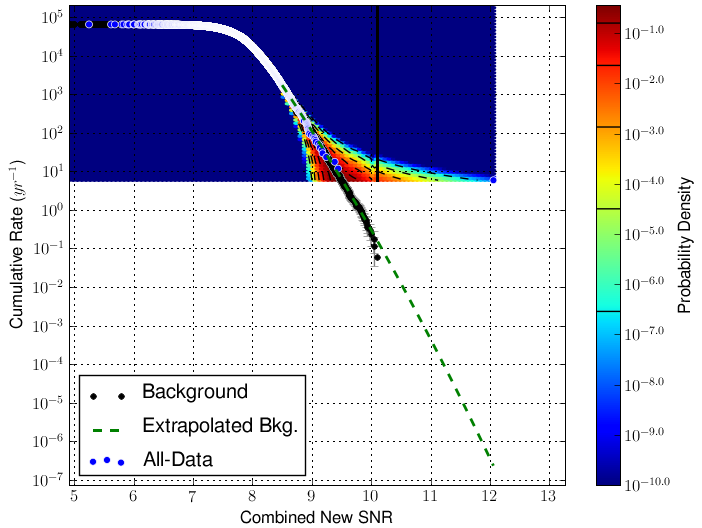
\includegraphics[height=3in]{figures/big_dog/plotrates-cum_hist_ext-low_mchirp_bin-S6CD.png}}
\subfigure[The medium chirp-mass bin.]{\label{fig:big_dog-cum_hist-extrap_med}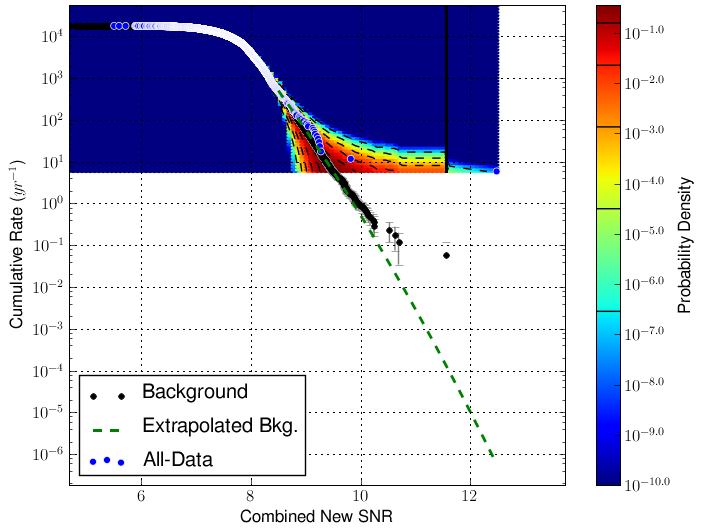
\includegraphics[height=3in]{figures/big_dog/plotrates-cum_hist_ext-med_mchirp_bin-S6CD.png}}
\caption{Cumulative histogram of all H1L1 triggers in S6C and D as a function
of combined new \ac{SNR} in the low and medium chirp-mass bins. Zero-lag
triggers are represented by blue dots; slide triggers are black. In order to
make the probability-density color map, the y axes were initially normalized by
$T_{\mathrm{exp}}/T_{\mathrm{f}}$, as in Figure
\ref{fig:big_dog-non_cum_hist-extrap}. All points were then divided by
$T_{\mathrm{f}}$ to put the y axis in units of inverse years. The error bars on
the slide triggers are calculated using equation \ref{eqn:err_FAR} in Chapter
\ref{ch:far}. See the text for details on how the probability density was
calculated. The green-dashed line shows the complimentary error function using
the fit results from Figures \ref{fig:big_dog-cum_hist-extrap}.}
\label{fig:big_dog-cum_hist-extrap}
\end{figure}

\begin{figure}[p]
\center
\subfigure[The low chirp-mass bin.]{\label{fig:big_dog-cum_hist_no_littles-extrap_low}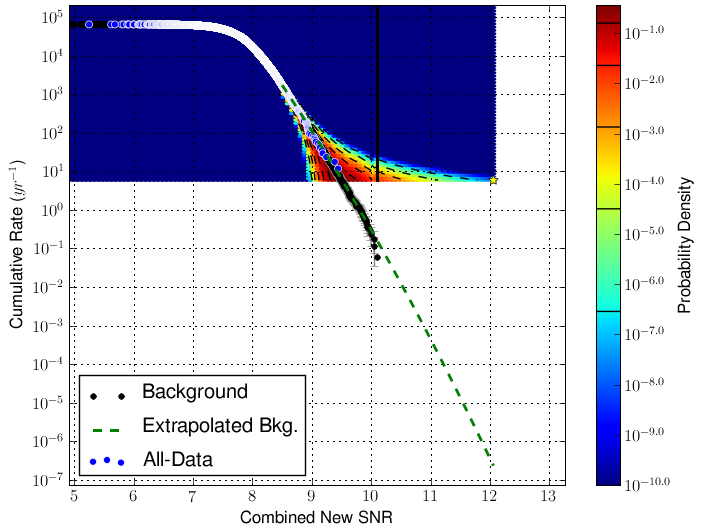
\includegraphics[height=3in]{figures/big_dog/plotrates-cum_hist_ext_no_littles-low_mchirp_bin-S6CD.png}}
\subfigure[The medium chirp-mass bin.]{\label{fig:big_dog-cum_hist_no_littles-extrap_med}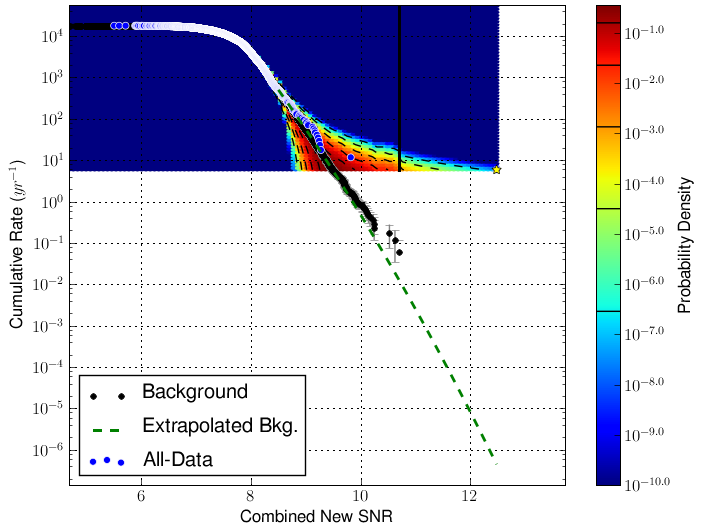
\includegraphics[height=3in]{figures/big_dog/plotrates-cum_hist_ext_no_littles-med_mchirp_bin-S6CD.png}}
\caption{Cumulative histograms with the blind injection excluded from the
time-slides. These plots are generated in the same manner as in Figure
\ref{fig:big_dog-cum_hist-extrap}. Here, the yellow star represents the blind
injection. A Gaussian was fitted to non-cumulative slide distributions with the
blind injection removed. The fit values were then used to create the
extrapolations, shown as the green-dashed line.}
\label{fig:big_dog-cum_hist_no_littles-extrap}
\end{figure}

\begin{figure}[p]
\center
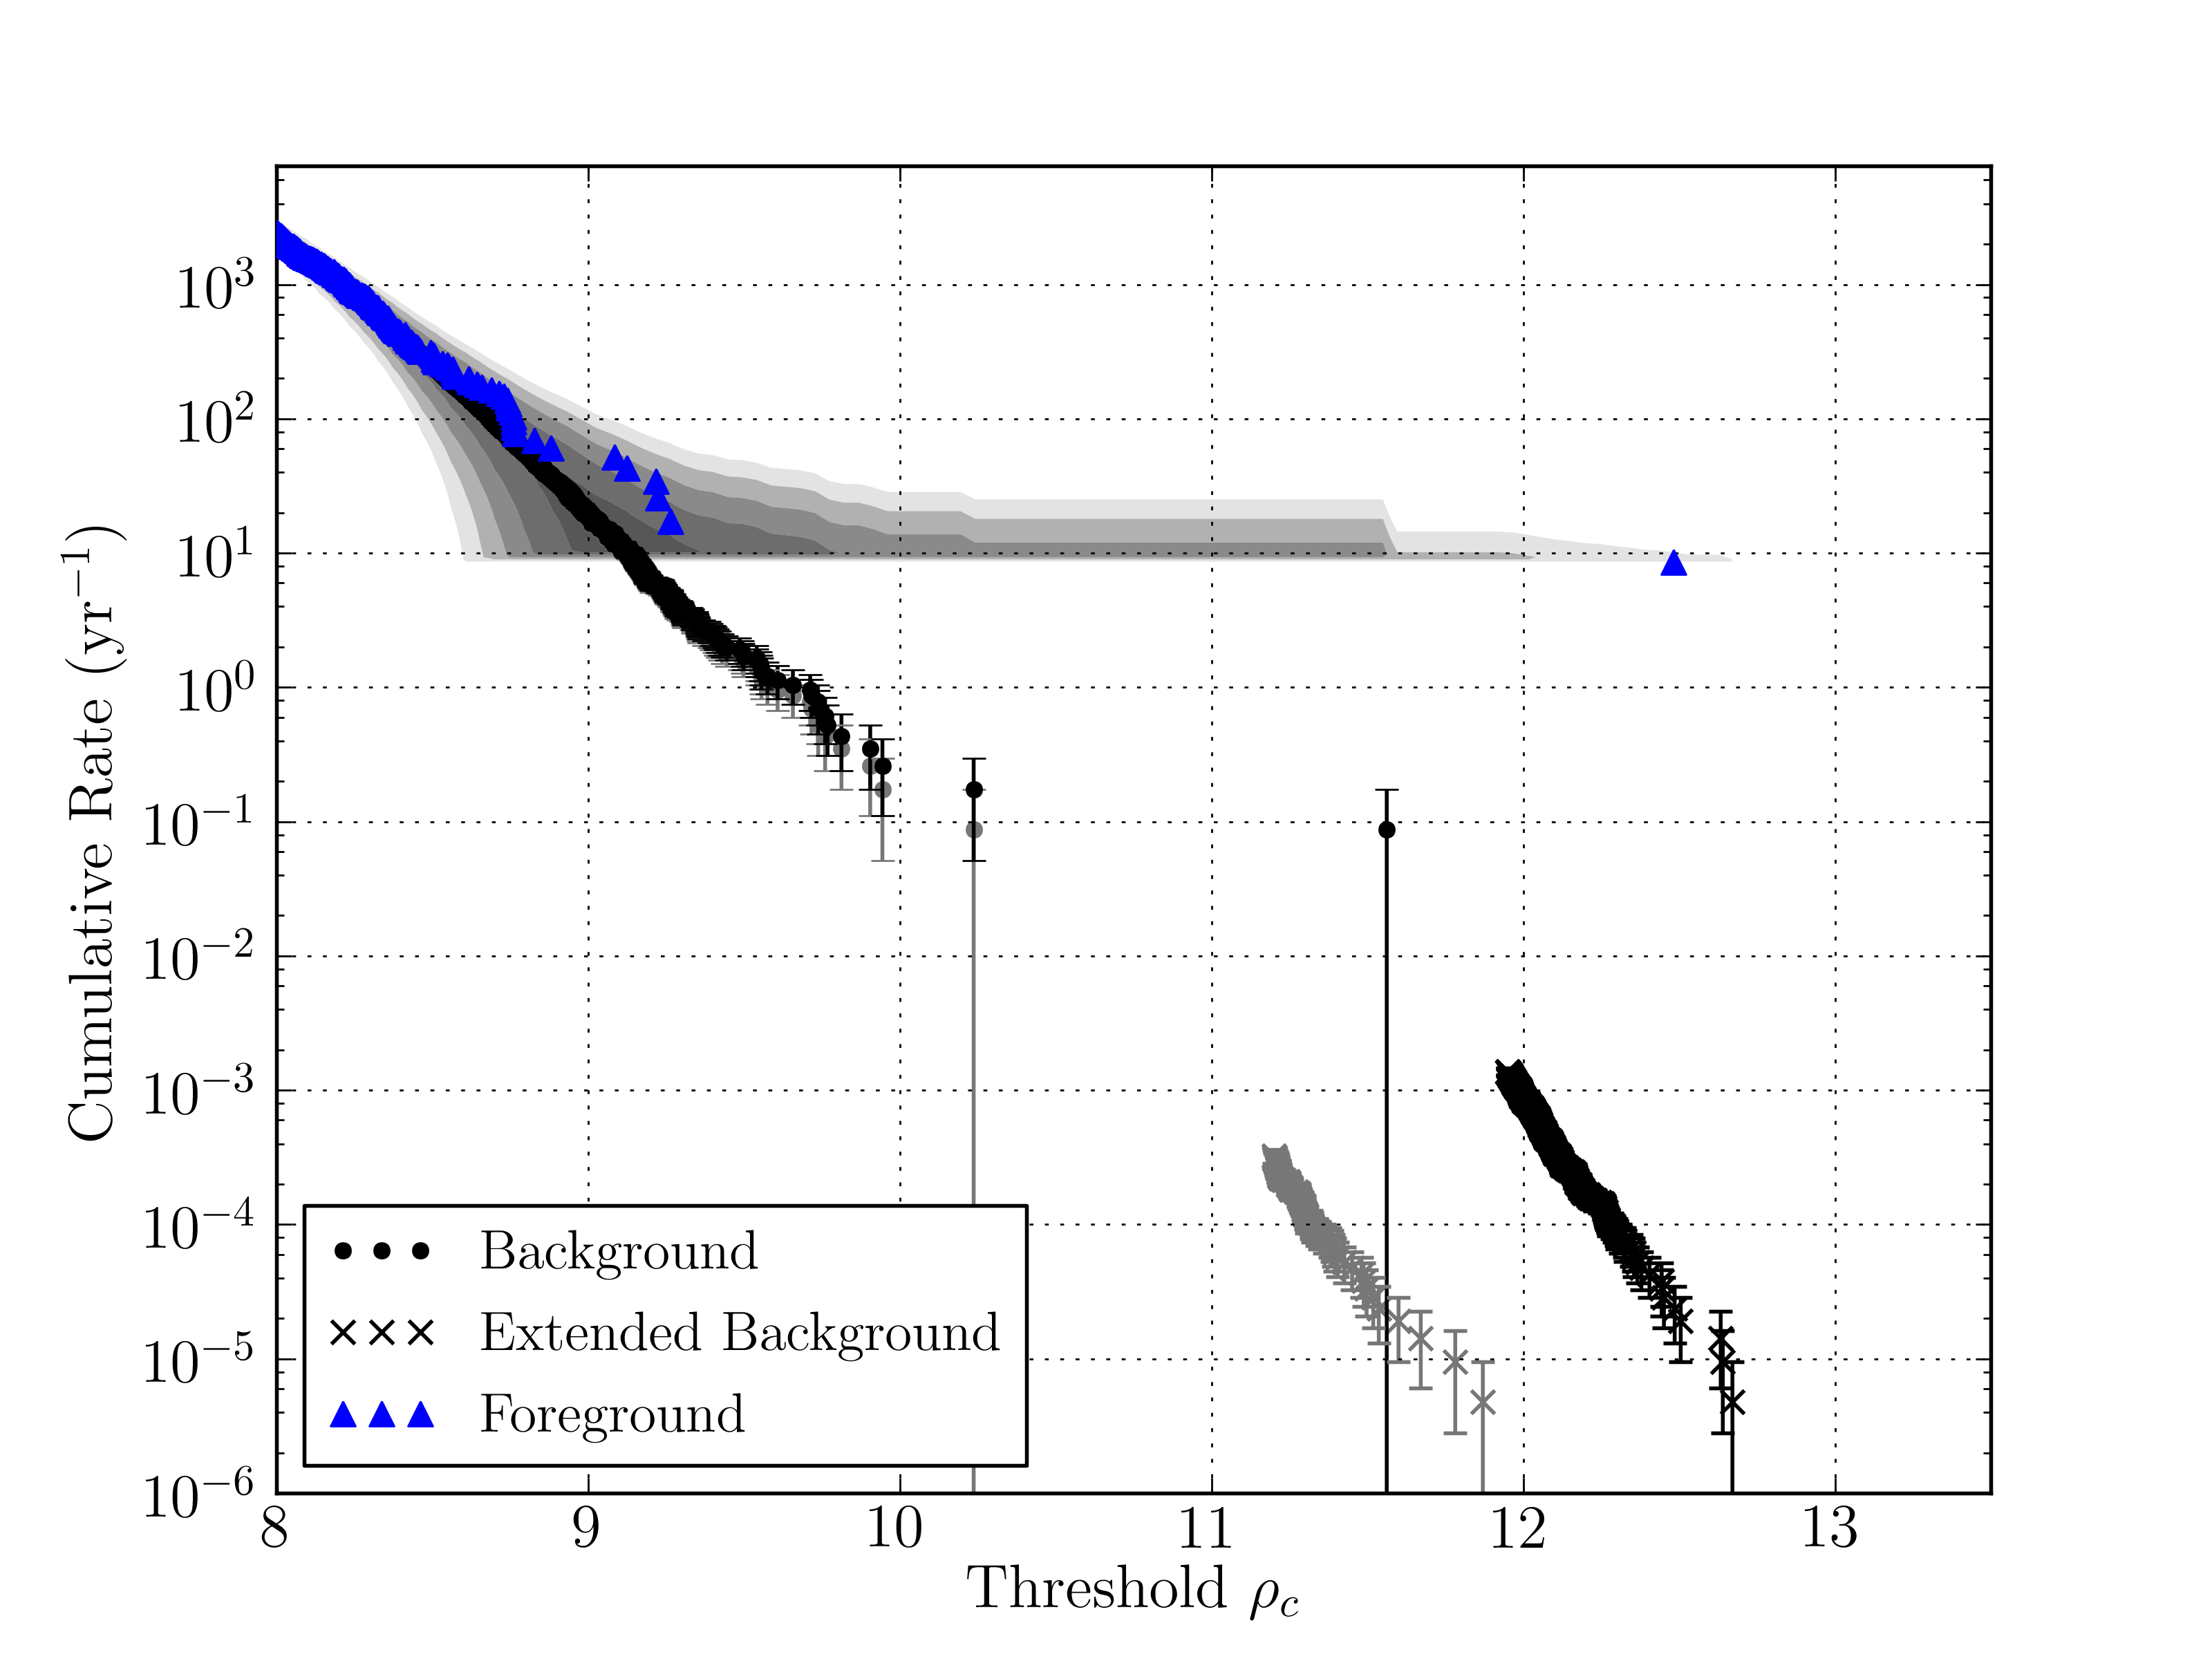
\includegraphics[width=6in]{figures/big_dog/H1L1V1-lalapps_cbc_plotrates_FINAL_PLOT_cumulative_F1_ALL_DATA_PLOTTED_OPEN_BOX-961545543-10076544.png}
\caption{The cumulative rate of H1L1 events with chirp mass $3.48 \le \mathcal{M}/\Msun
< 7.40$ in S6D as a function of combined New SNR (here, labeled
``Threshold $\rho_c$"). This plot was generated in a manner similar to the
Figures \ref{fig:big_dog-cum_hist-extrap} and
\ref{fig:big_dog-cum_hist_no_littles-extrap}, except that no extrapolation was
done. We have also replaced the probability density color map by the gray
shaded contours, which show the $1 - 5\sigma$ (dark to light) regions of the
PDF. The blue triangles show coincident events.  Black dots show the
background estimated from 100 time shifts and black crosses show the extended
background estimation from all possible 5-second shifts on this data.  The gray
dots and crosses show the corresponding background estimates when a $\pm 8$
seconds of data around the time of the blind injection are excluded. Had the
blind injection been real, this plot would have been one of the main figures of
merit used in the detection paper.}
\label{fig:big_dog-rate_plot}
\end{figure}
